\documentclass[journal, a4paper]{IEEEtran}
\usepackage[italian]{babel}
\usepackage{booktabs}
\usepackage{siunitx}%Questo serve a caricare il pacchetto delle unità di misura del sistema internazionale%
\usepackage[utf8]{inputenc}
\usepackage{graphicx} 
\usepackage{url}
\usepackage{amsmath}
\usepackage{amssymb}


\usepackage{keyval}
\usepackage{xcolor}
\usepackage{caption}
\usepackage{subfig}
\usepackage{tikz}
\usepackage{circuitikz}
\usepackage{authblk}
%\usepackage{hyperref}

\begin{document}


% Define document title and author
	\title{Tecnologie Digitali - Logbook Week 14}
	\author[1]{Salvatore Bottaro}
		\author[2]{Lorenzo M. Perrone}
		\affil[1]{\texttt{salvo.bottaro@hotmail.it}}
		\affil[2]{\texttt{lorenzo.perrone.lmp@gmail.com}}
	\markboth{Tecnologie Digitali - Di Lieto}{}
	\maketitle
	
\begin{abstract}
	Logbook di laboratorio di Tecnologie Digitali, a.a. 2015/2016. Week 14
\end{abstract}

[Es.9] Scegliamo adesso come tensione di alimentazione del partitore 1:10 quella fornita direttamente da \textsc{Arduino} sul pin \textbf{Aref} del microcontrollore. La tensione effettiva misurata col tester digitale è di $V_{ref} = 5.04(4) \si{V}$, quella in uscita dal partitore (sempre con il tester) è $V_P = 530(4) \si{mV}$. Le acquisizioni con Arduino restituiscono un valore di n={104,105}, che corrisponderebbero ad un range di tensioni di 512-517 mV. Per stimare la dispersione delle misure, sono state effettuate circa 1150 acquisizioni distribuite come l'istogramma in Figura (\ref{fig:ist_DEFAULT_part105V}). La media delle misure è $V_{ave} = 104.99 = 517.25 \si{mV}$, mentre invece la deviazione standard è $\sigma = 0.01 = 0.05 \si{mV}$. L'incertezza dovuta alla risoluzione della misura, tuttavia, è di circa 5mV. Si nota una certa discrepanza rispetto i valori misurati col multimetro che distano circa 3 volte l'errore di risoluzione dal dato fornito da Arduino.\\

\begin{figure}
\centering
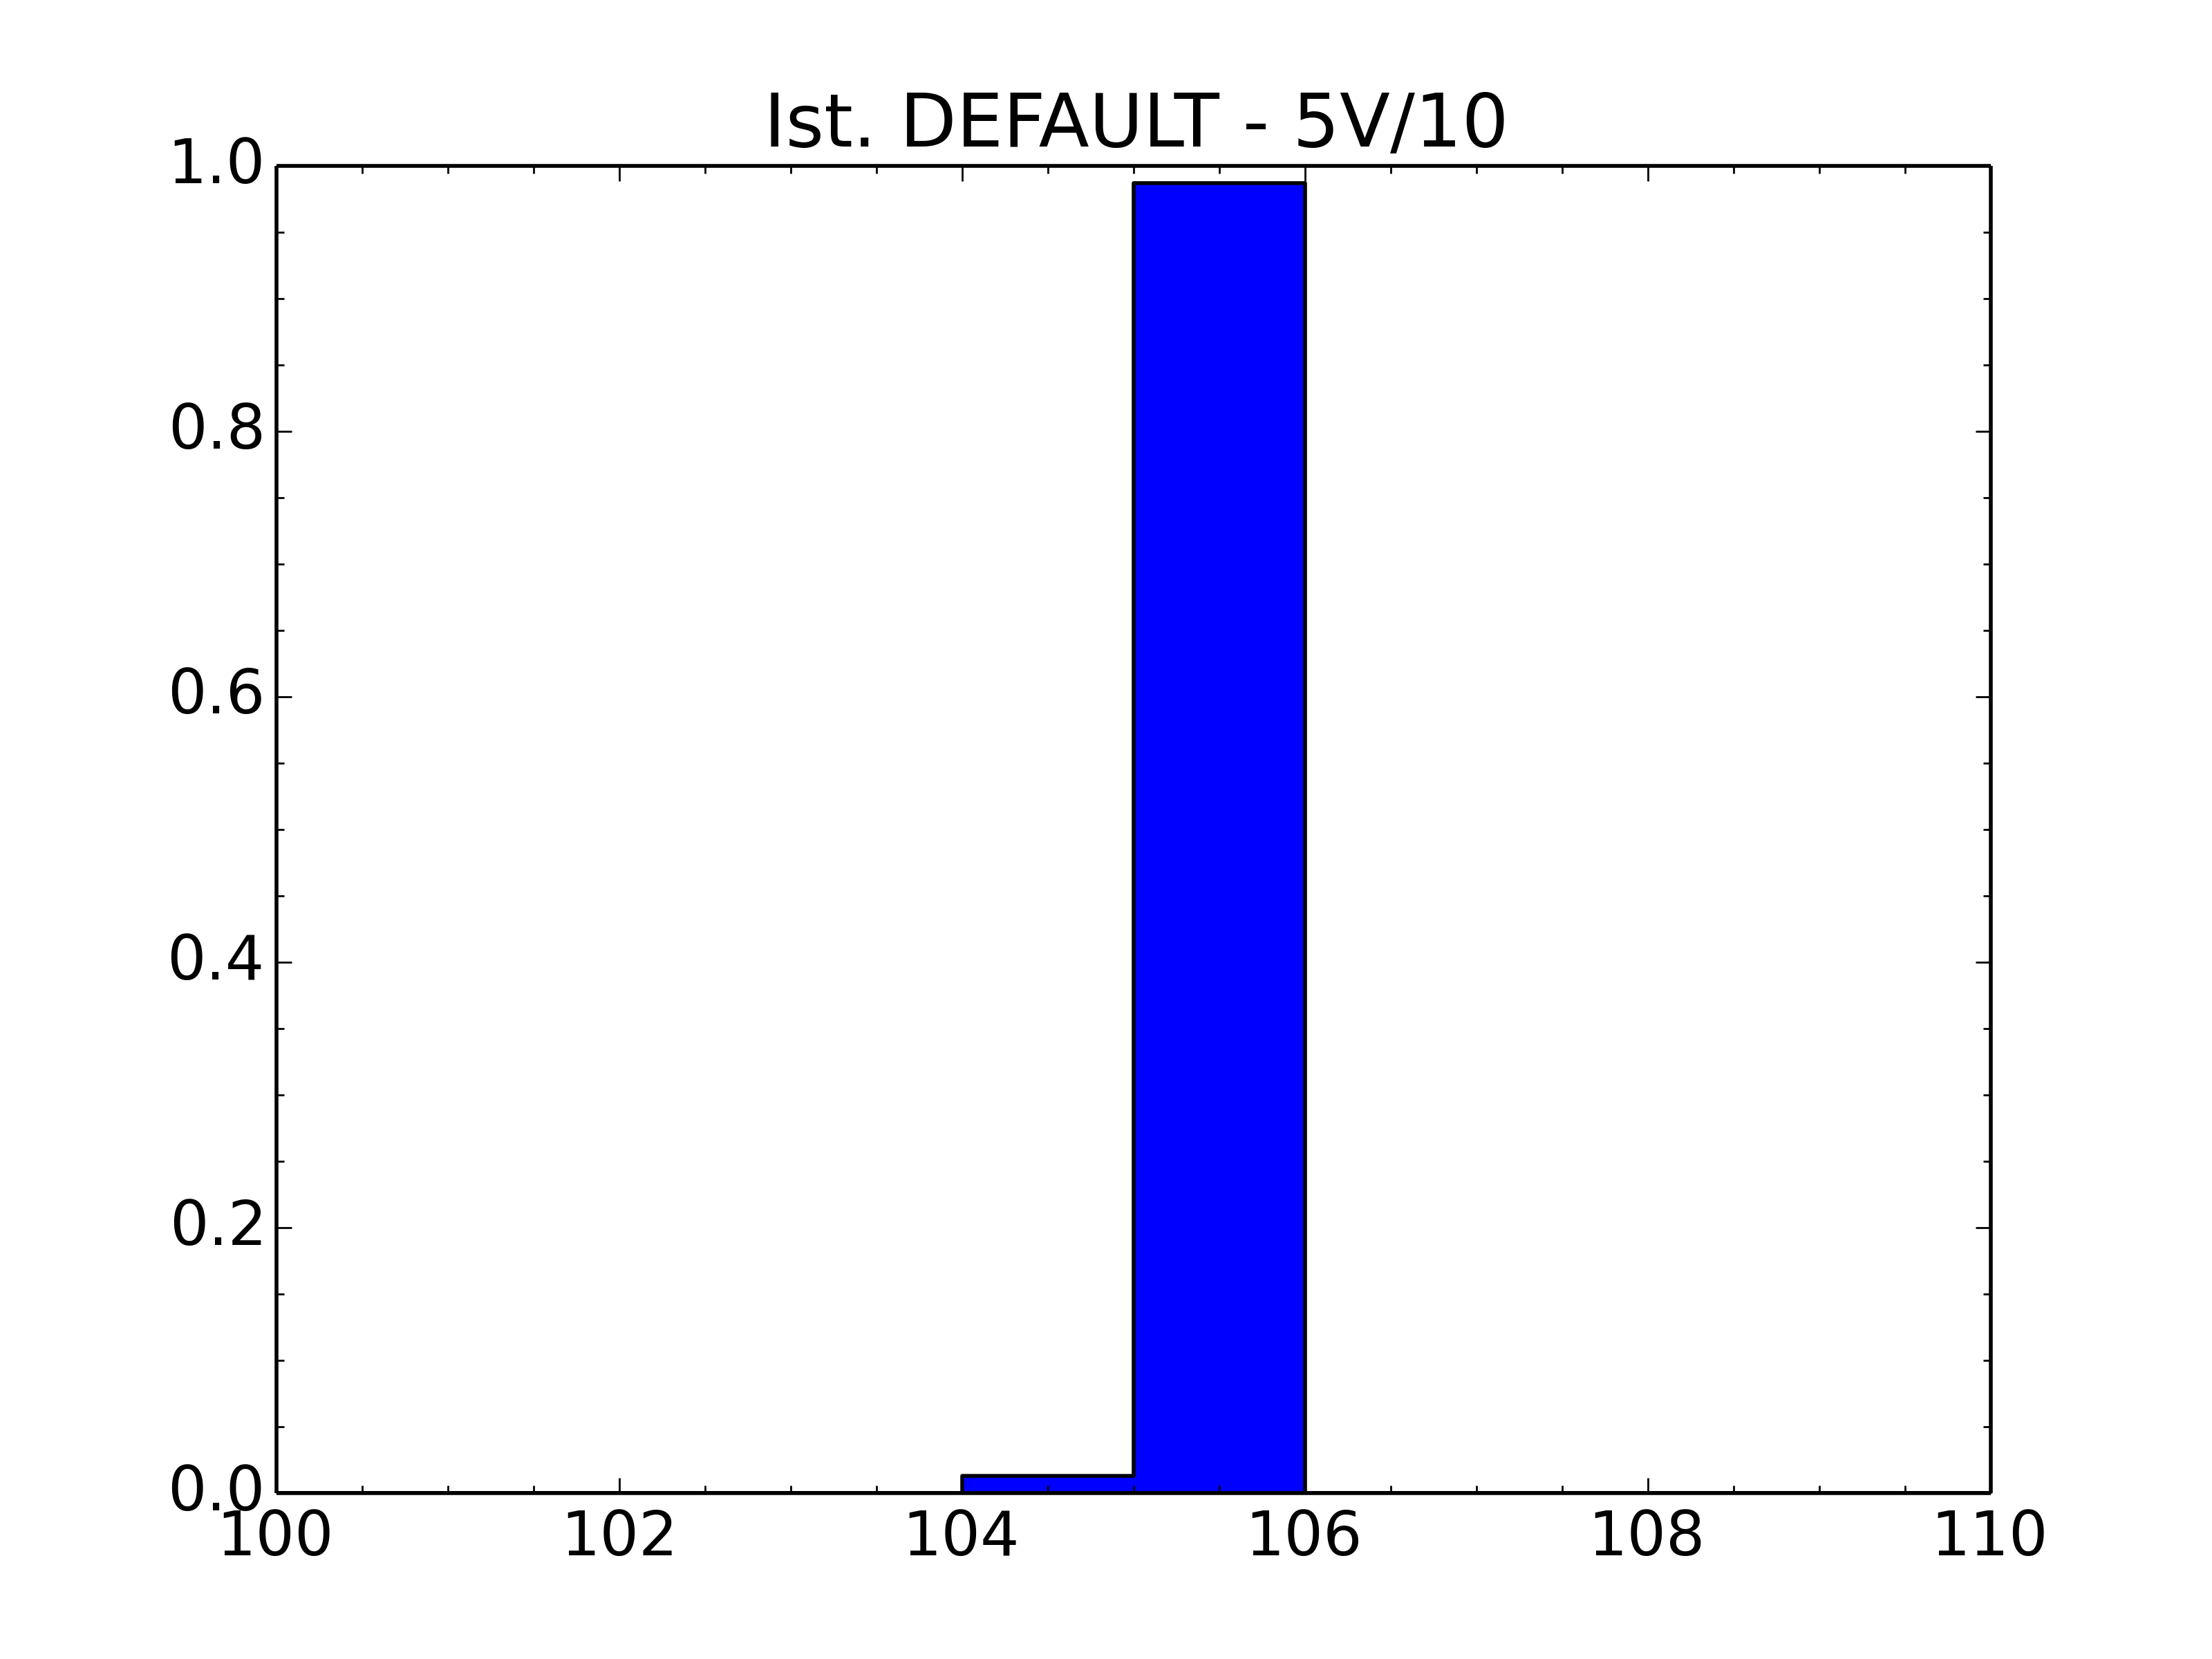
\includegraphics[width=0.9\linewidth]{./ist_DEFAULT_part105V}
\caption{Istogramma delle tensioni: Vin=Vref = 5V, partitore 1:10.}
\label{fig:ist_DEFAULT_part105V}
\end{figure}

Proviamo ora a modificare la tensione di riferimento di Arduino passando da \textsc{default} a \textsc{internal}: quest'ultima si riferisce ad un valore di 1.1V (nominali). Ciò permetterebbe una migliore risoluzione nella lettura delle tensioni in uscita dal partitore, che quindi sarebbero più precise. Tale risoluzione sarà infatti di 1mV. Proviamo a leggere con questa scala l'output del partitore (che ricordiamo è sempre collegato alla Aref): il risultato che ci aspettiamo sarà sempre dell'ordine di n={104,105}, probabilmente distribuito in maniera differente rispetto al caso precedente. L'istogramma è in Figura (\ref{fig:ist_INTERNAL_part10_1V}).\\

\begin{figure}
\centering
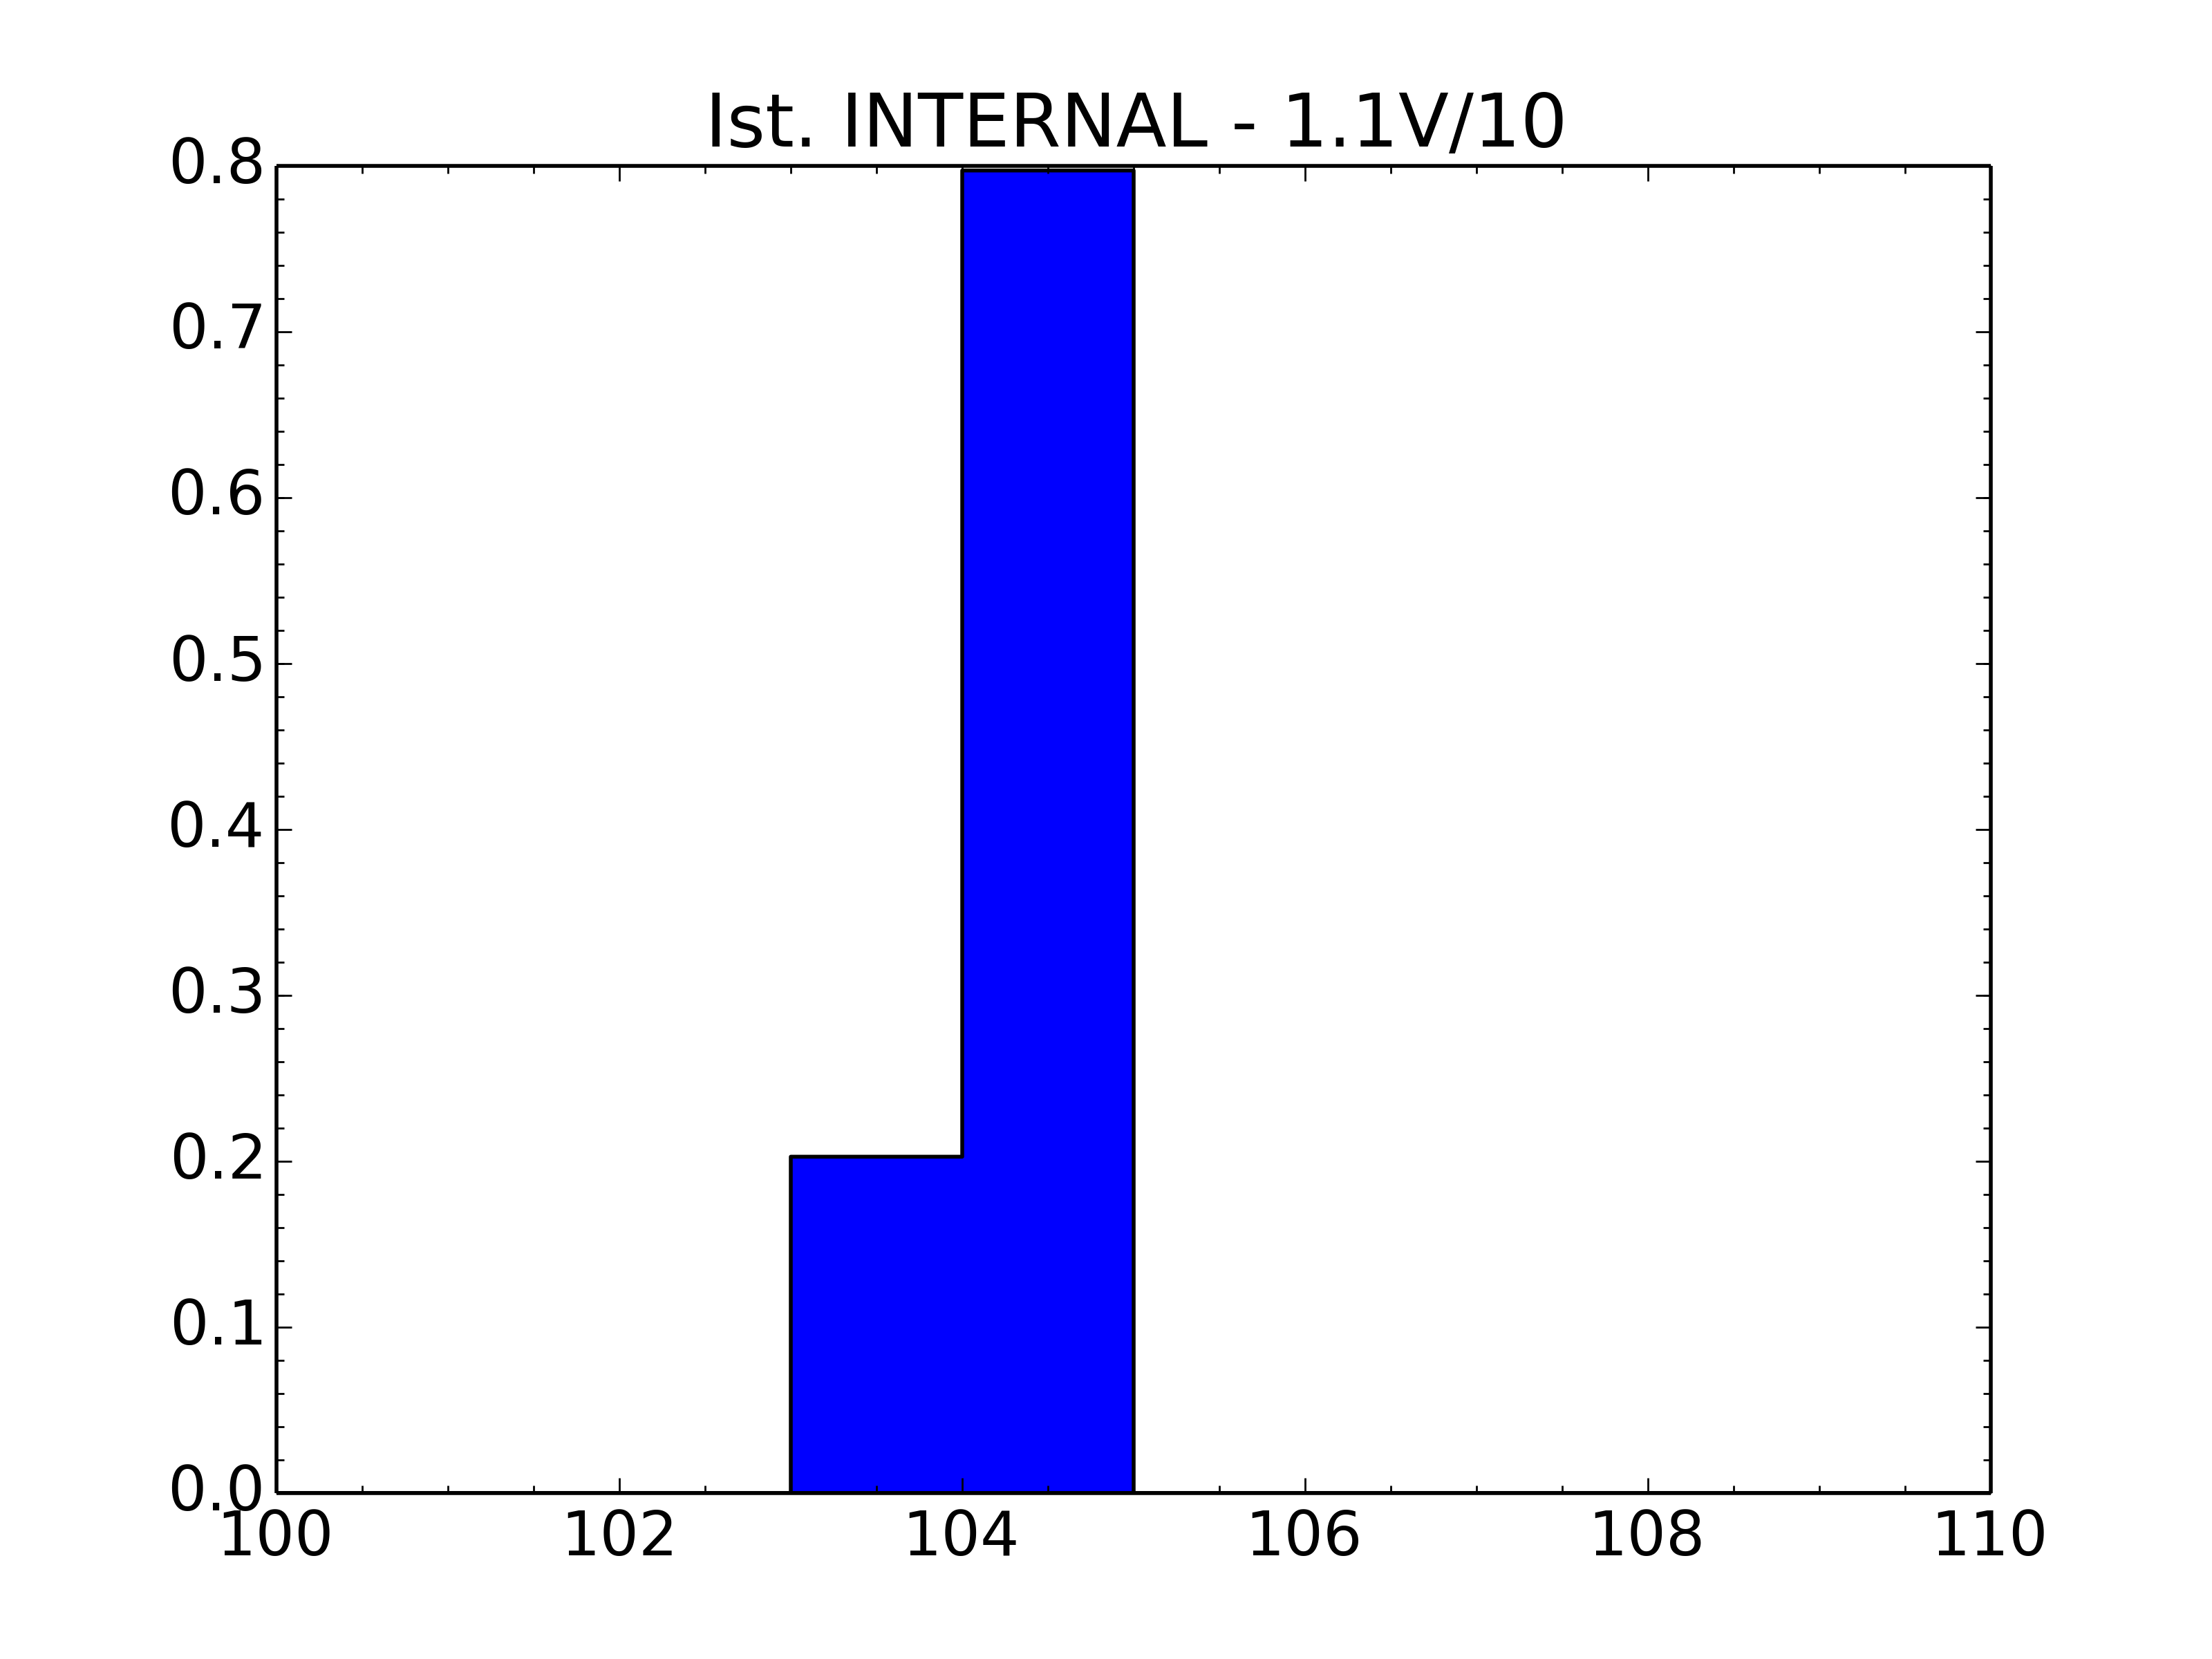
\includegraphics[width=0.9\linewidth]{./ist_INTERNAL_part10_1V}
\caption{Istogramma delle tensioni: Vin=Vref=1.1V, partitore 1:10.}
\label{fig:ist_INTERNAL_part10_1V}
\end{figure}

Gli n restituiti sono {103,104}, anche se questa volta le due popolazioni sono dello stesso ordine di grandezza. Per convertire il dato in tensioni, abbiamo misurato con il multimetro la porta Aref ottenendo $V_{ref} = 1.07$V. Il range di tensioni è 108-109 mV, la media e la deviazione standard sono rispettivamente: 103.8(2) , che convertito in tensione risulta 108.6(2) mV. In base al rapporto del nostro partitore ci saremmo aspettati, tuttavia, un valore di circa 125mV che dista sempre di circa 15mV da quello misurato.\\


Concludiamo queste prove lasciando sempre come tensione di riferimento la \textsc{internal}, ma fornendo al partitore i 5V presi dal pin 2 del connettore delle alimentazioni. Andremo a confrontare questo dato (e la sua variabilità) con quello ottenuto nel primo istogramma. Il numero di campionamenti effettuato è di circa 800, e i risultati sono presentati in Figura (\ref{fig:ist_INTERNAL_part10_5V}). Come possiamo notare, la variabilità di n è decisamente più alta della prima situazione considerata, vi sono infatti 4 valori di n campionati: n={506,507,508,509}. Il range di tensione è dunque: 529-532 mV. La media di 530.5(2) mV.

\begin{figure}
\centering
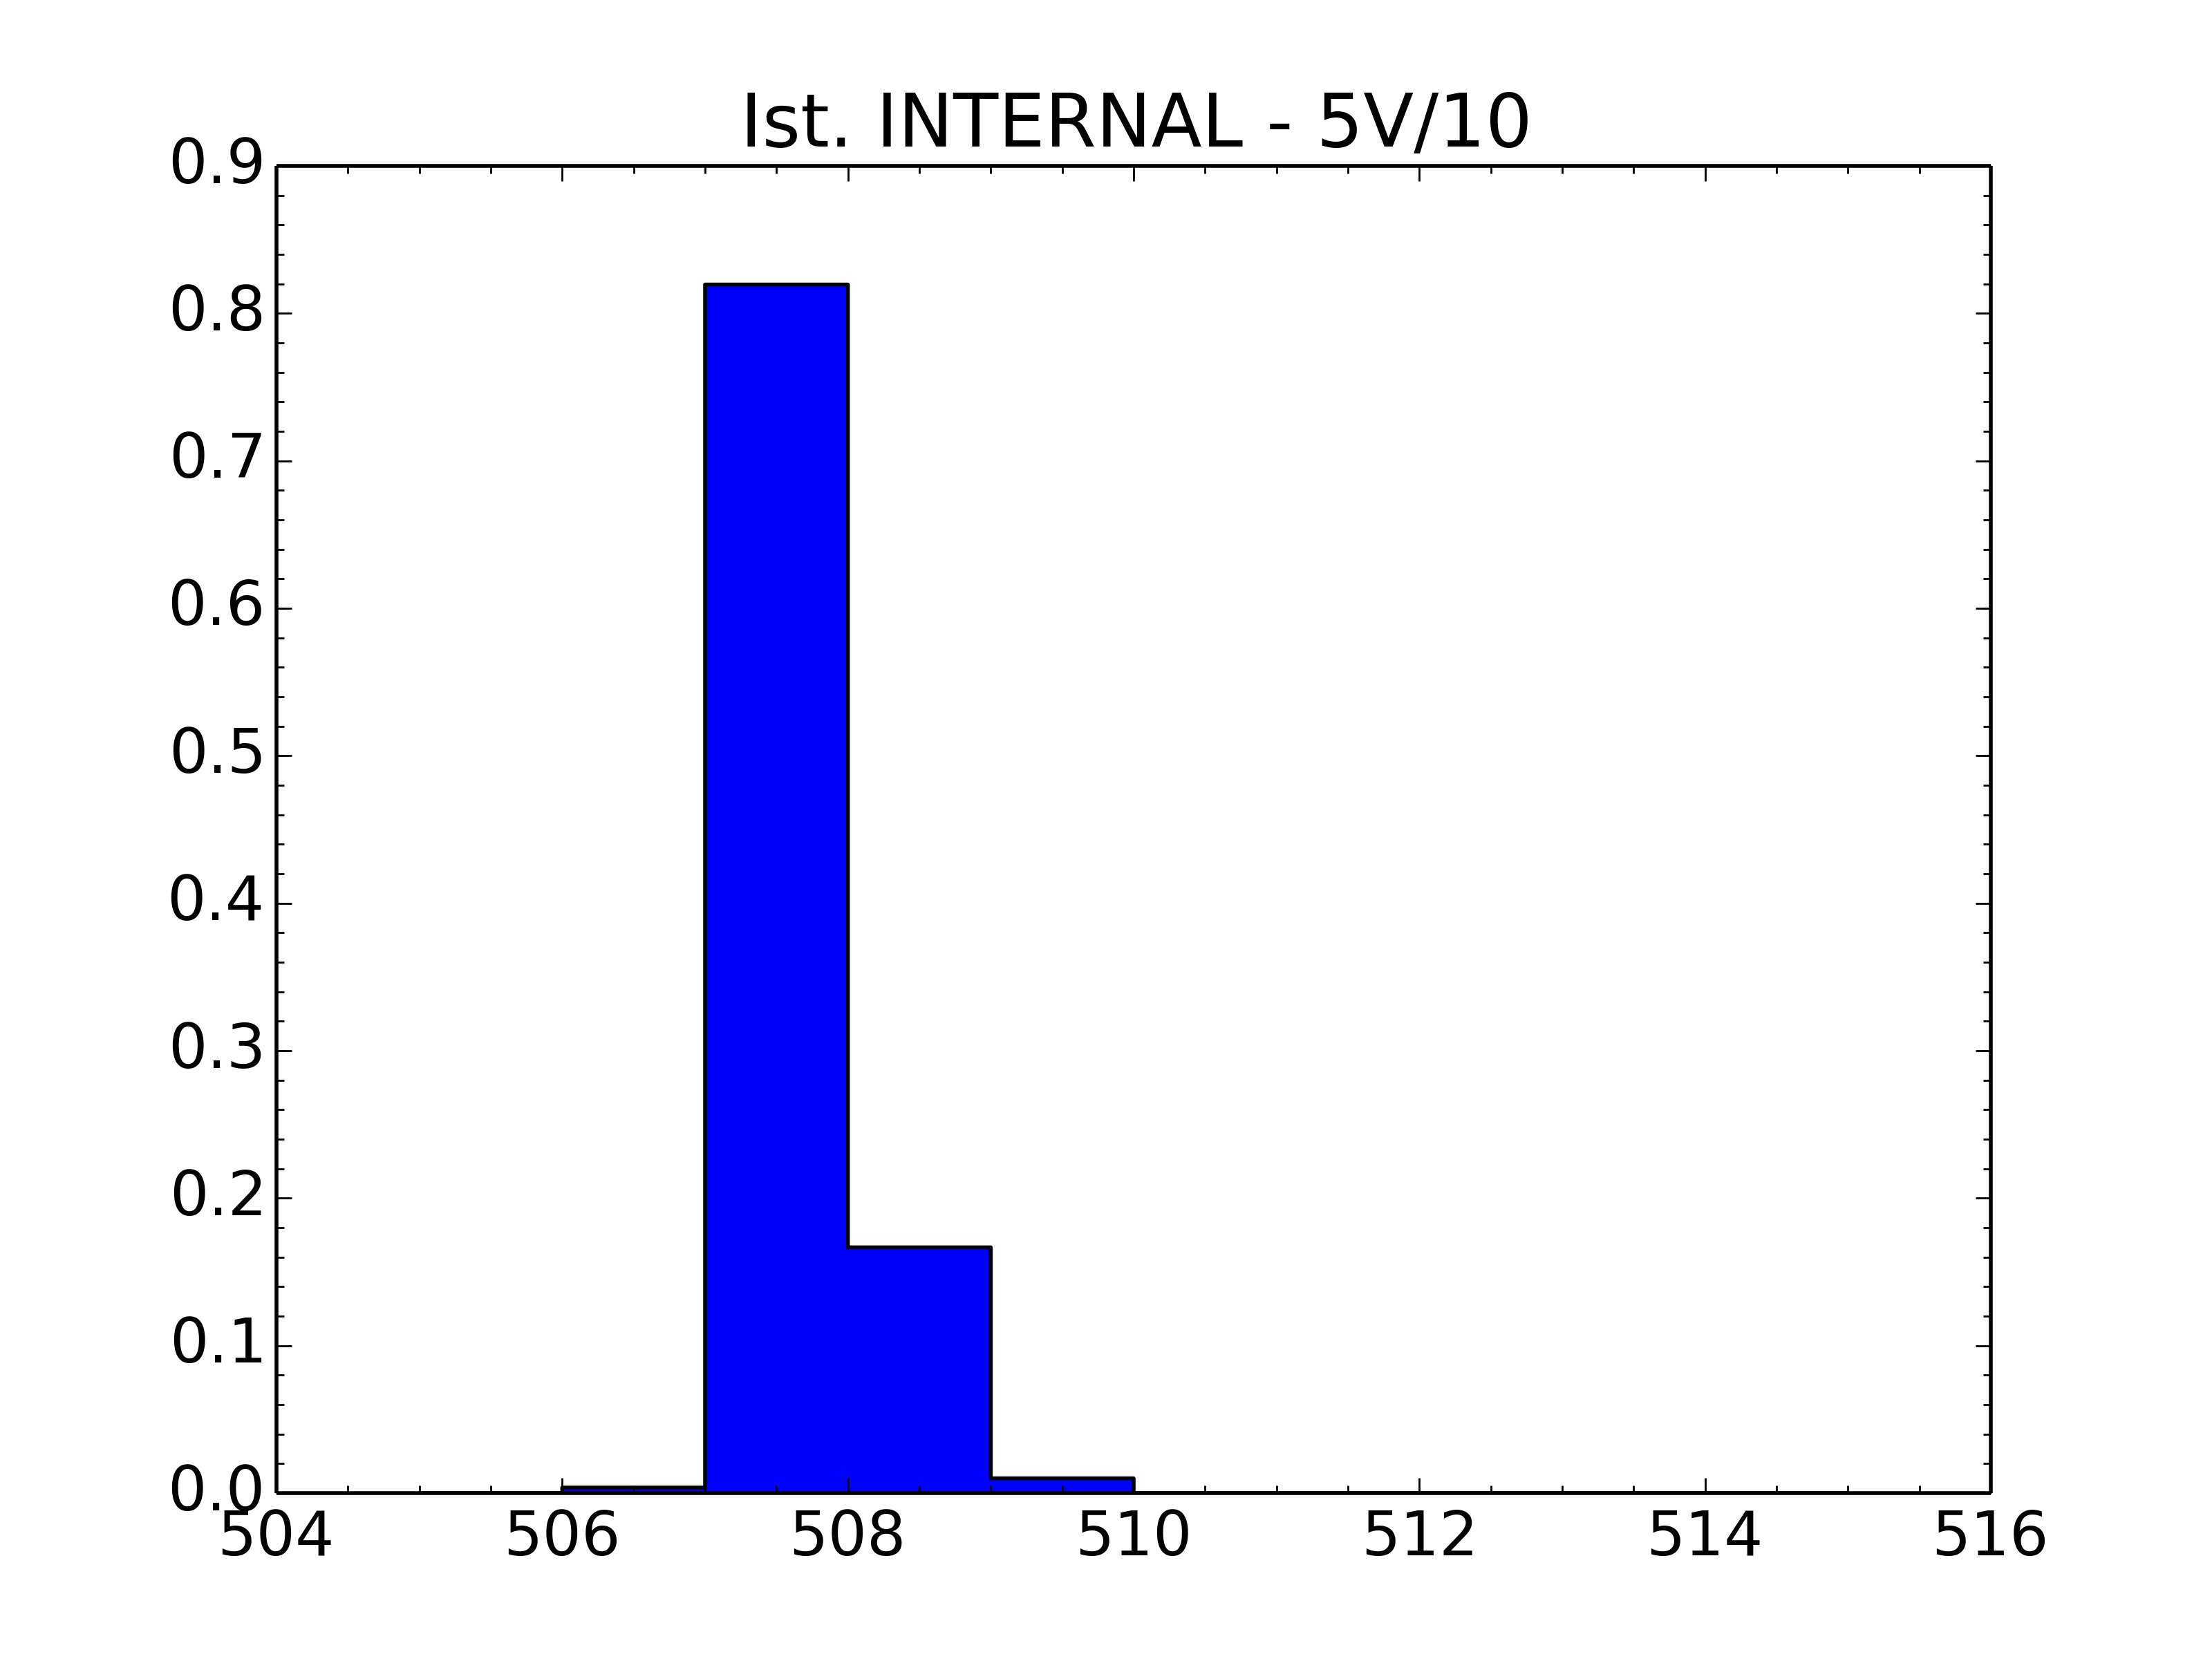
\includegraphics[width=0.9\linewidth]{./ist_INTERNAL_part10_5V}
\caption{Istogramma delle tensioni: Vref = 1.1V, Vin = 5V, partitore 1:10}
\label{fig:ist_INTERNAL_part10_5V}
\end{figure}

\section{Velocità del convertitore ADC interno}

Imppostiamo un segnale di frequenza 4Hz sul generatore di funzioni, con ampiezza picco picco $V_{PP} = 4$V e offset = +2.5V, in modo tale da rimanere sempre di mezzo volt al di sotto della soglia di 5V e al di sopra del livello di terra. Campioniamo con \textsc{acquis\_base} il segnale sinusoidale per verificare che le impostazioni siano corrette: come si vede dalla Figura (\ref{fig:es11_provaacquisbase}), il risultato è molto buono.\\

\begin{figure}
\centering
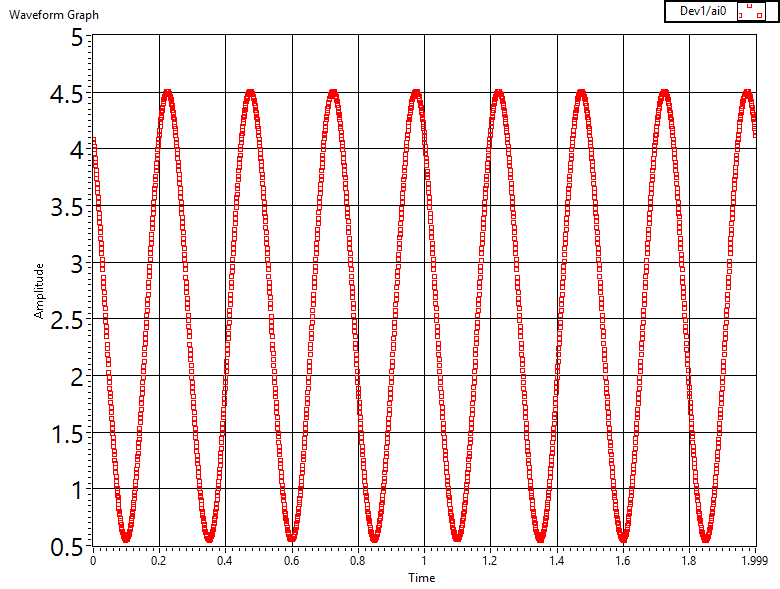
\includegraphics[width=0.9\linewidth]{./es11_provaacquisbase}
\caption{Segnale sinusoidale - ACQUIS\_BASE}
\label{fig:es11_provaacquisbase}
\end{figure}

\begin{figure}
\centering
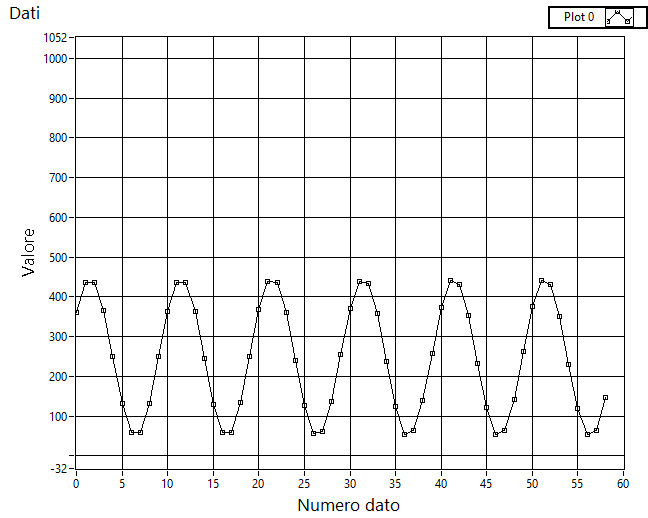
\includegraphics[width=0.7\linewidth]{./es11_1hz_100ms}
\caption{Segnale 1Hz, ARDUINO}
\label{fig:es11_1hz_100ms}
\end{figure}

Proviamo adesso a utilizzare Arduino per leggere le tensioni in uscita al partitore 1:10 con un segnale di ingresso di questo tipo (in realtà la frequenza è stata abbassata a 1Hz). I livelli di tensione sono abbastanza ben rispettati e la sinusoide è ben riconoscibile (Figura (\ref{fig:es11_1hz_100ms})). Riportando a 4Hz la frequenza del seno, invece, si notano dei pattern molto simili a quelli visibili con il fenomeno dei battimenti, come se ci fosse una seconda frequenza in gioco (vedi Figura (\ref{fig:es11_4hz_100ms})). In realtà, questo fenomeno è dovuto essenzialmente al basso numero di campionamenti per singolo periodo , dovuti al delay di 100ms impostato nello sketch: ARDUINO campiona circa 2 punti per ogni periodo, in punti sempre diversi dell'onda poichè le frequenze non sono in rapporto intero fra loro. \\
Una riprova di questa spiegazione è stata ottenuta simulando un segnale sinusoidale con Python e campionandolo con punti piuttosto radi lungo un gran numero di periodi. I risultati che si possono ottenere giocando con l'intervallo di campionamento sono mostrati nelle Figure (\ref{fig:soluzione_es11_1batt}-\ref{fig:soluzione_es11_2batt}-\ref{fig:soluzione_es11_3batt}).\\


\begin{figure}
\centering
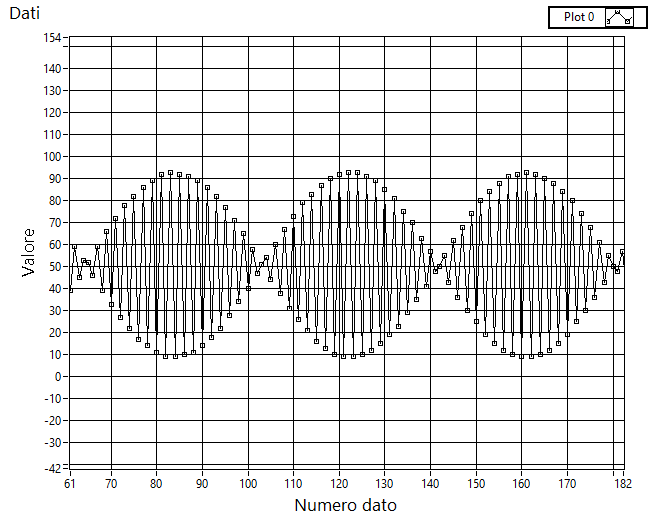
\includegraphics[width=0.7\linewidth]{./es11_4hz_100ms}
\caption{Forma del segnale a 4Hz aquisito con ARDUINO}
\label{fig:es11_4hz_100ms}
\end{figure}

\begin{figure}
\centering
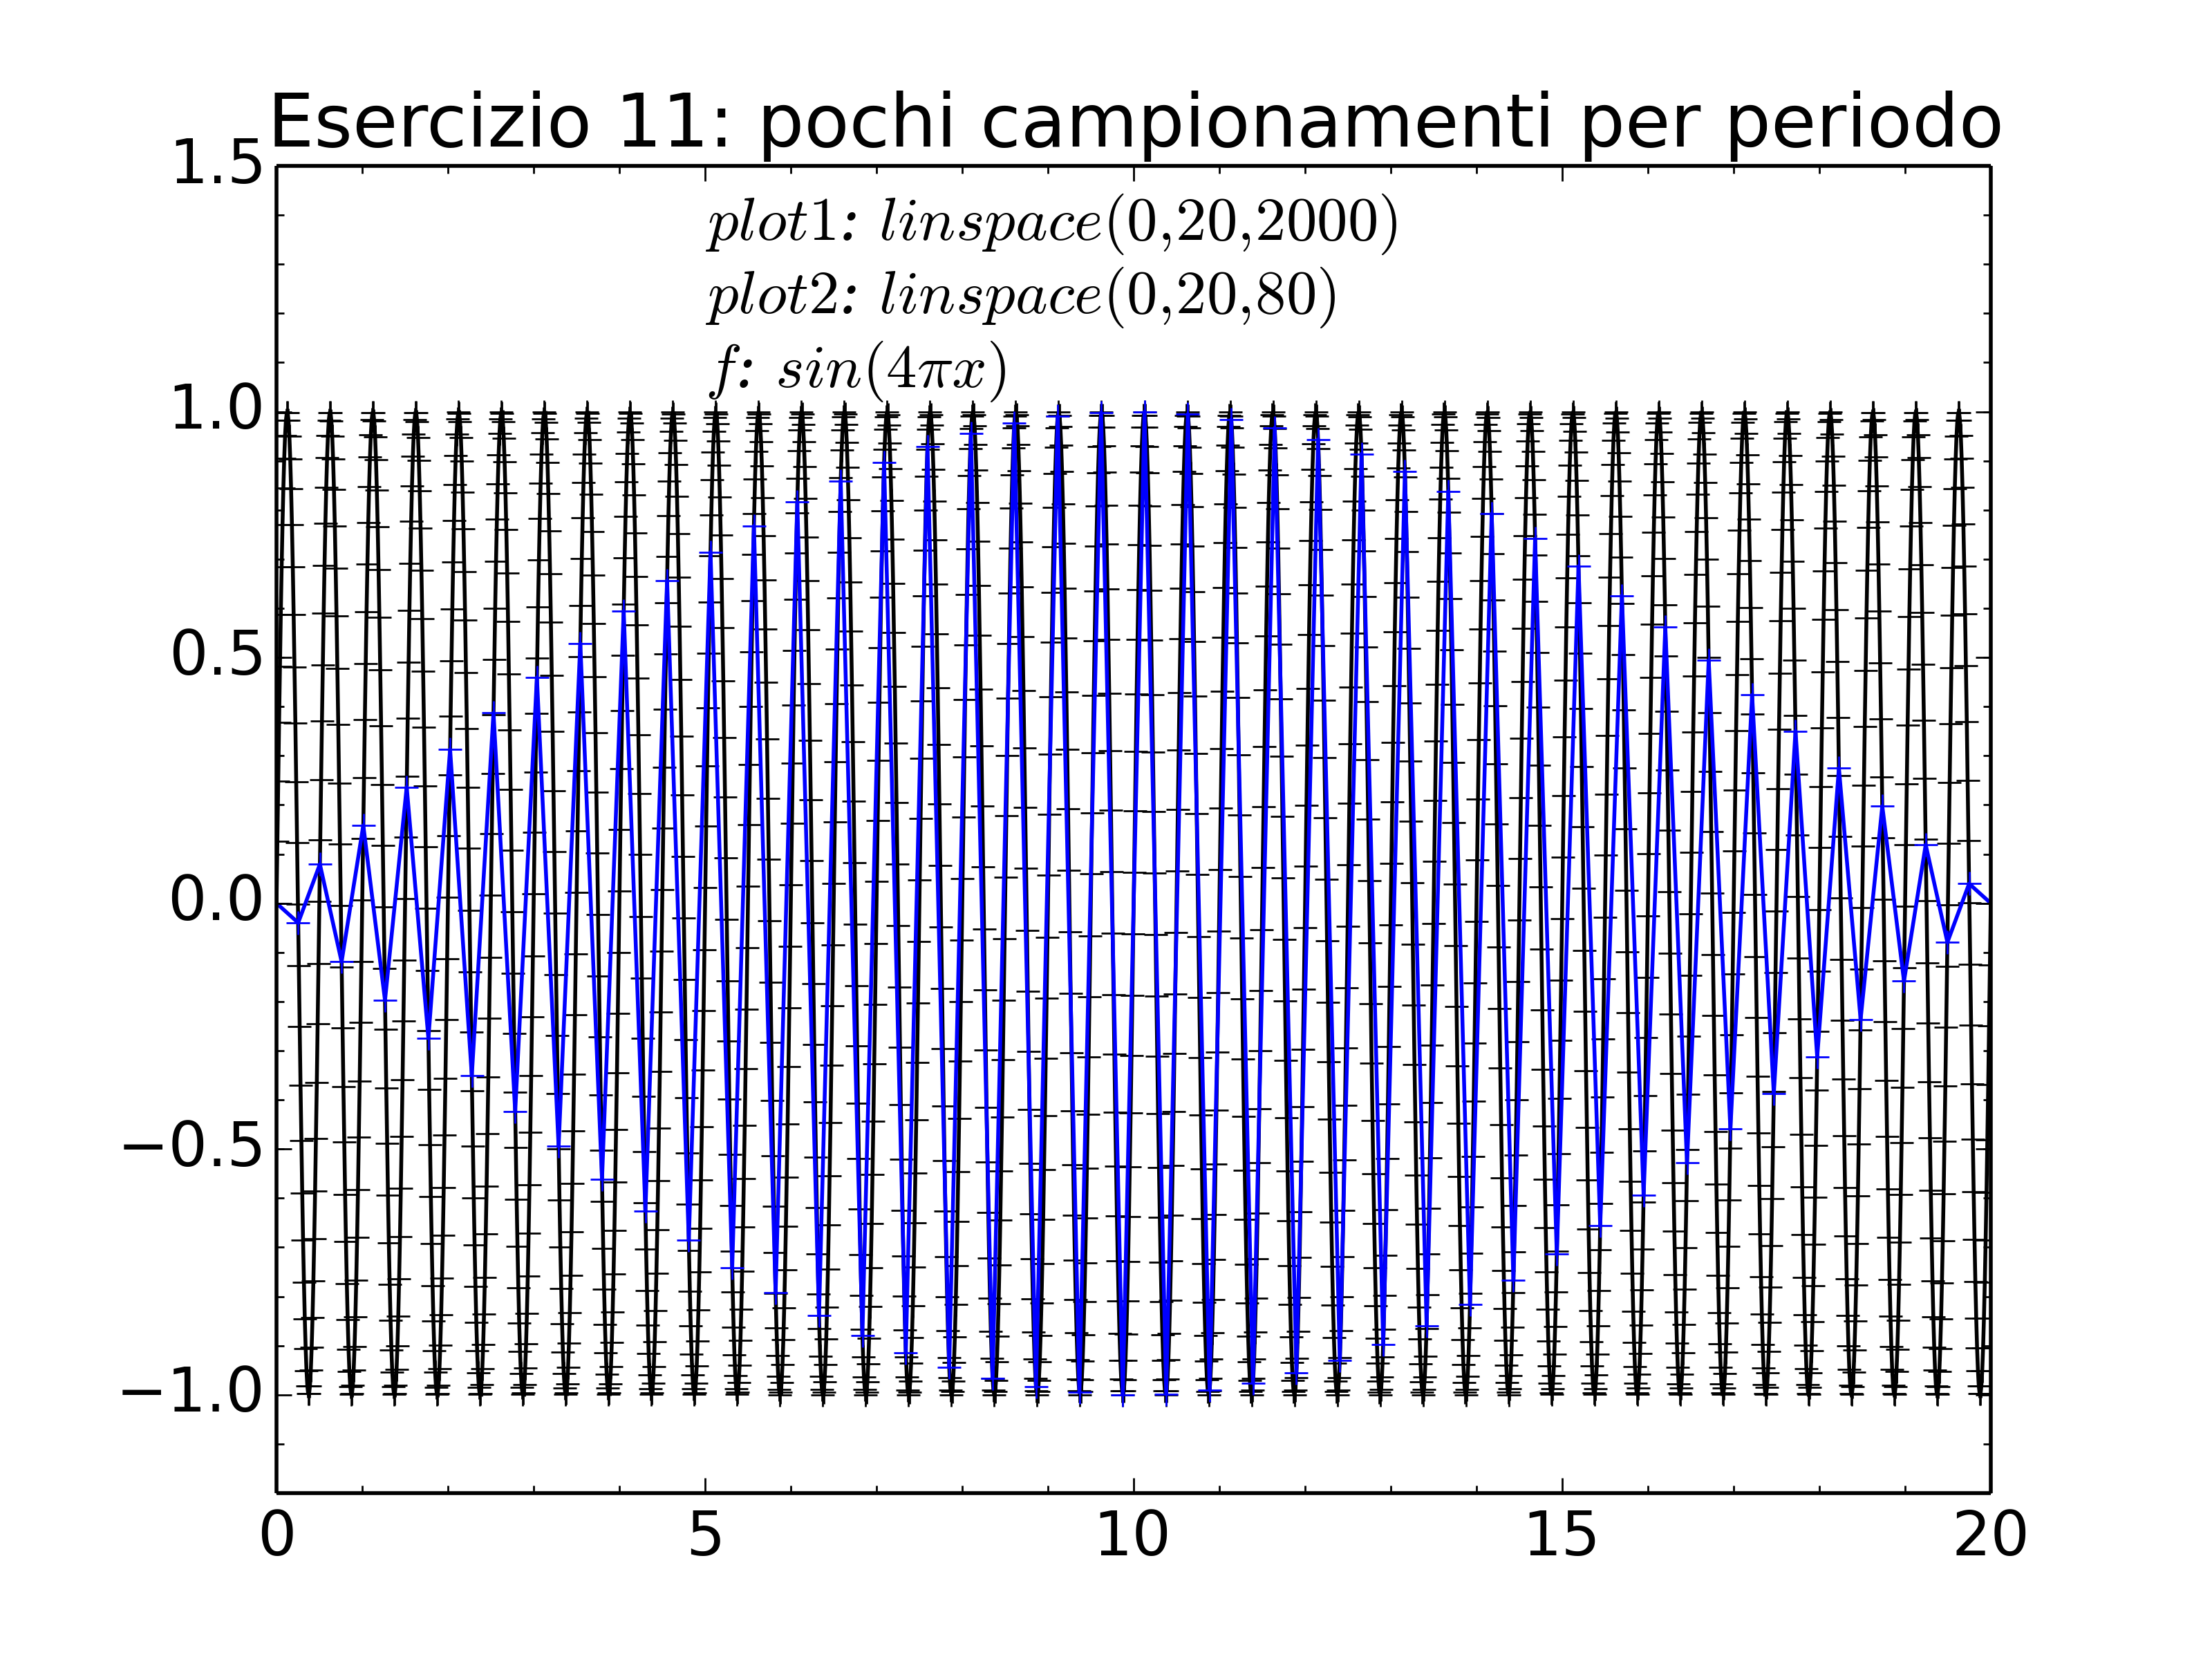
\includegraphics[width=0.9\linewidth]{./soluzione_es11_1batt}
\caption{Forma d'onda ottenuta dal campionamento di un segnale sinusoidale, acquisendo pochi dati per periodo}
\label{fig:soluzione_es11_1batt}
\end{figure}

\begin{figure}
\centering
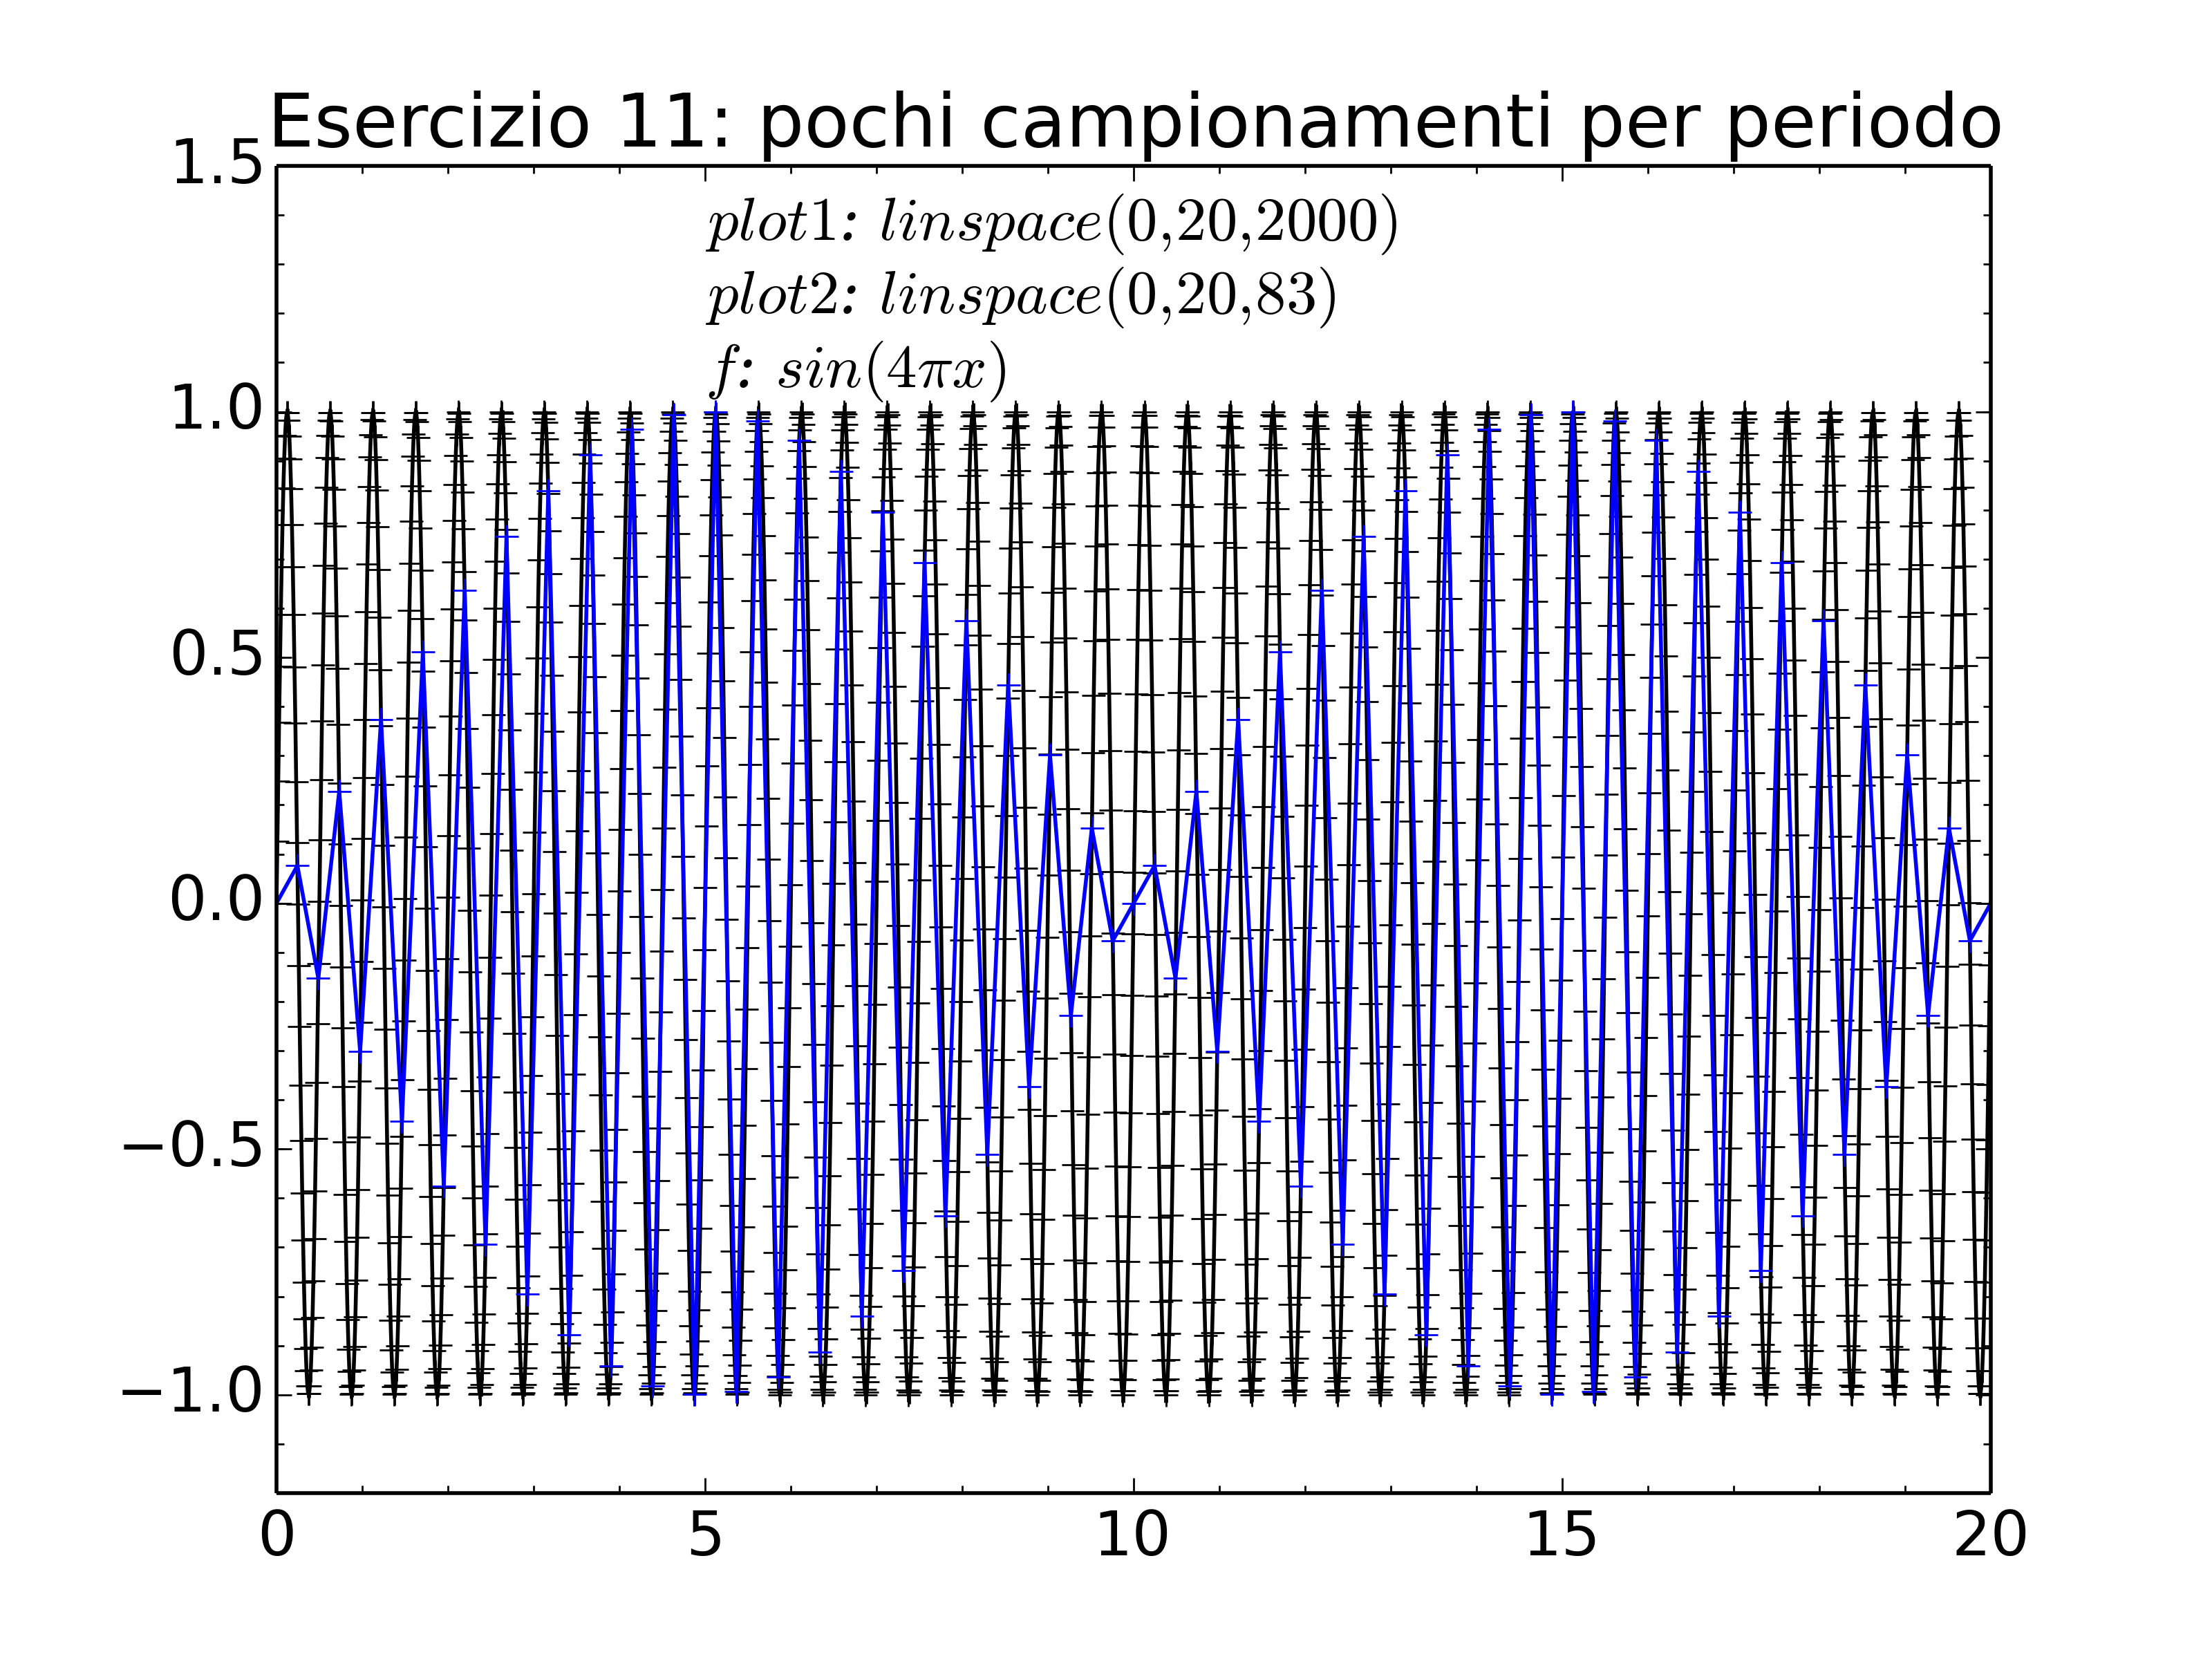
\includegraphics[width=0.9\linewidth]{./soluzione_es11_2batt}
\caption{Forma d'onda ottenuta dal campionamento di un segnale sinusoidale, acquisendo pochi dati per periodo}
\label{fig:soluzione_es11_2batt}
\end{figure}

\begin{figure}
\centering
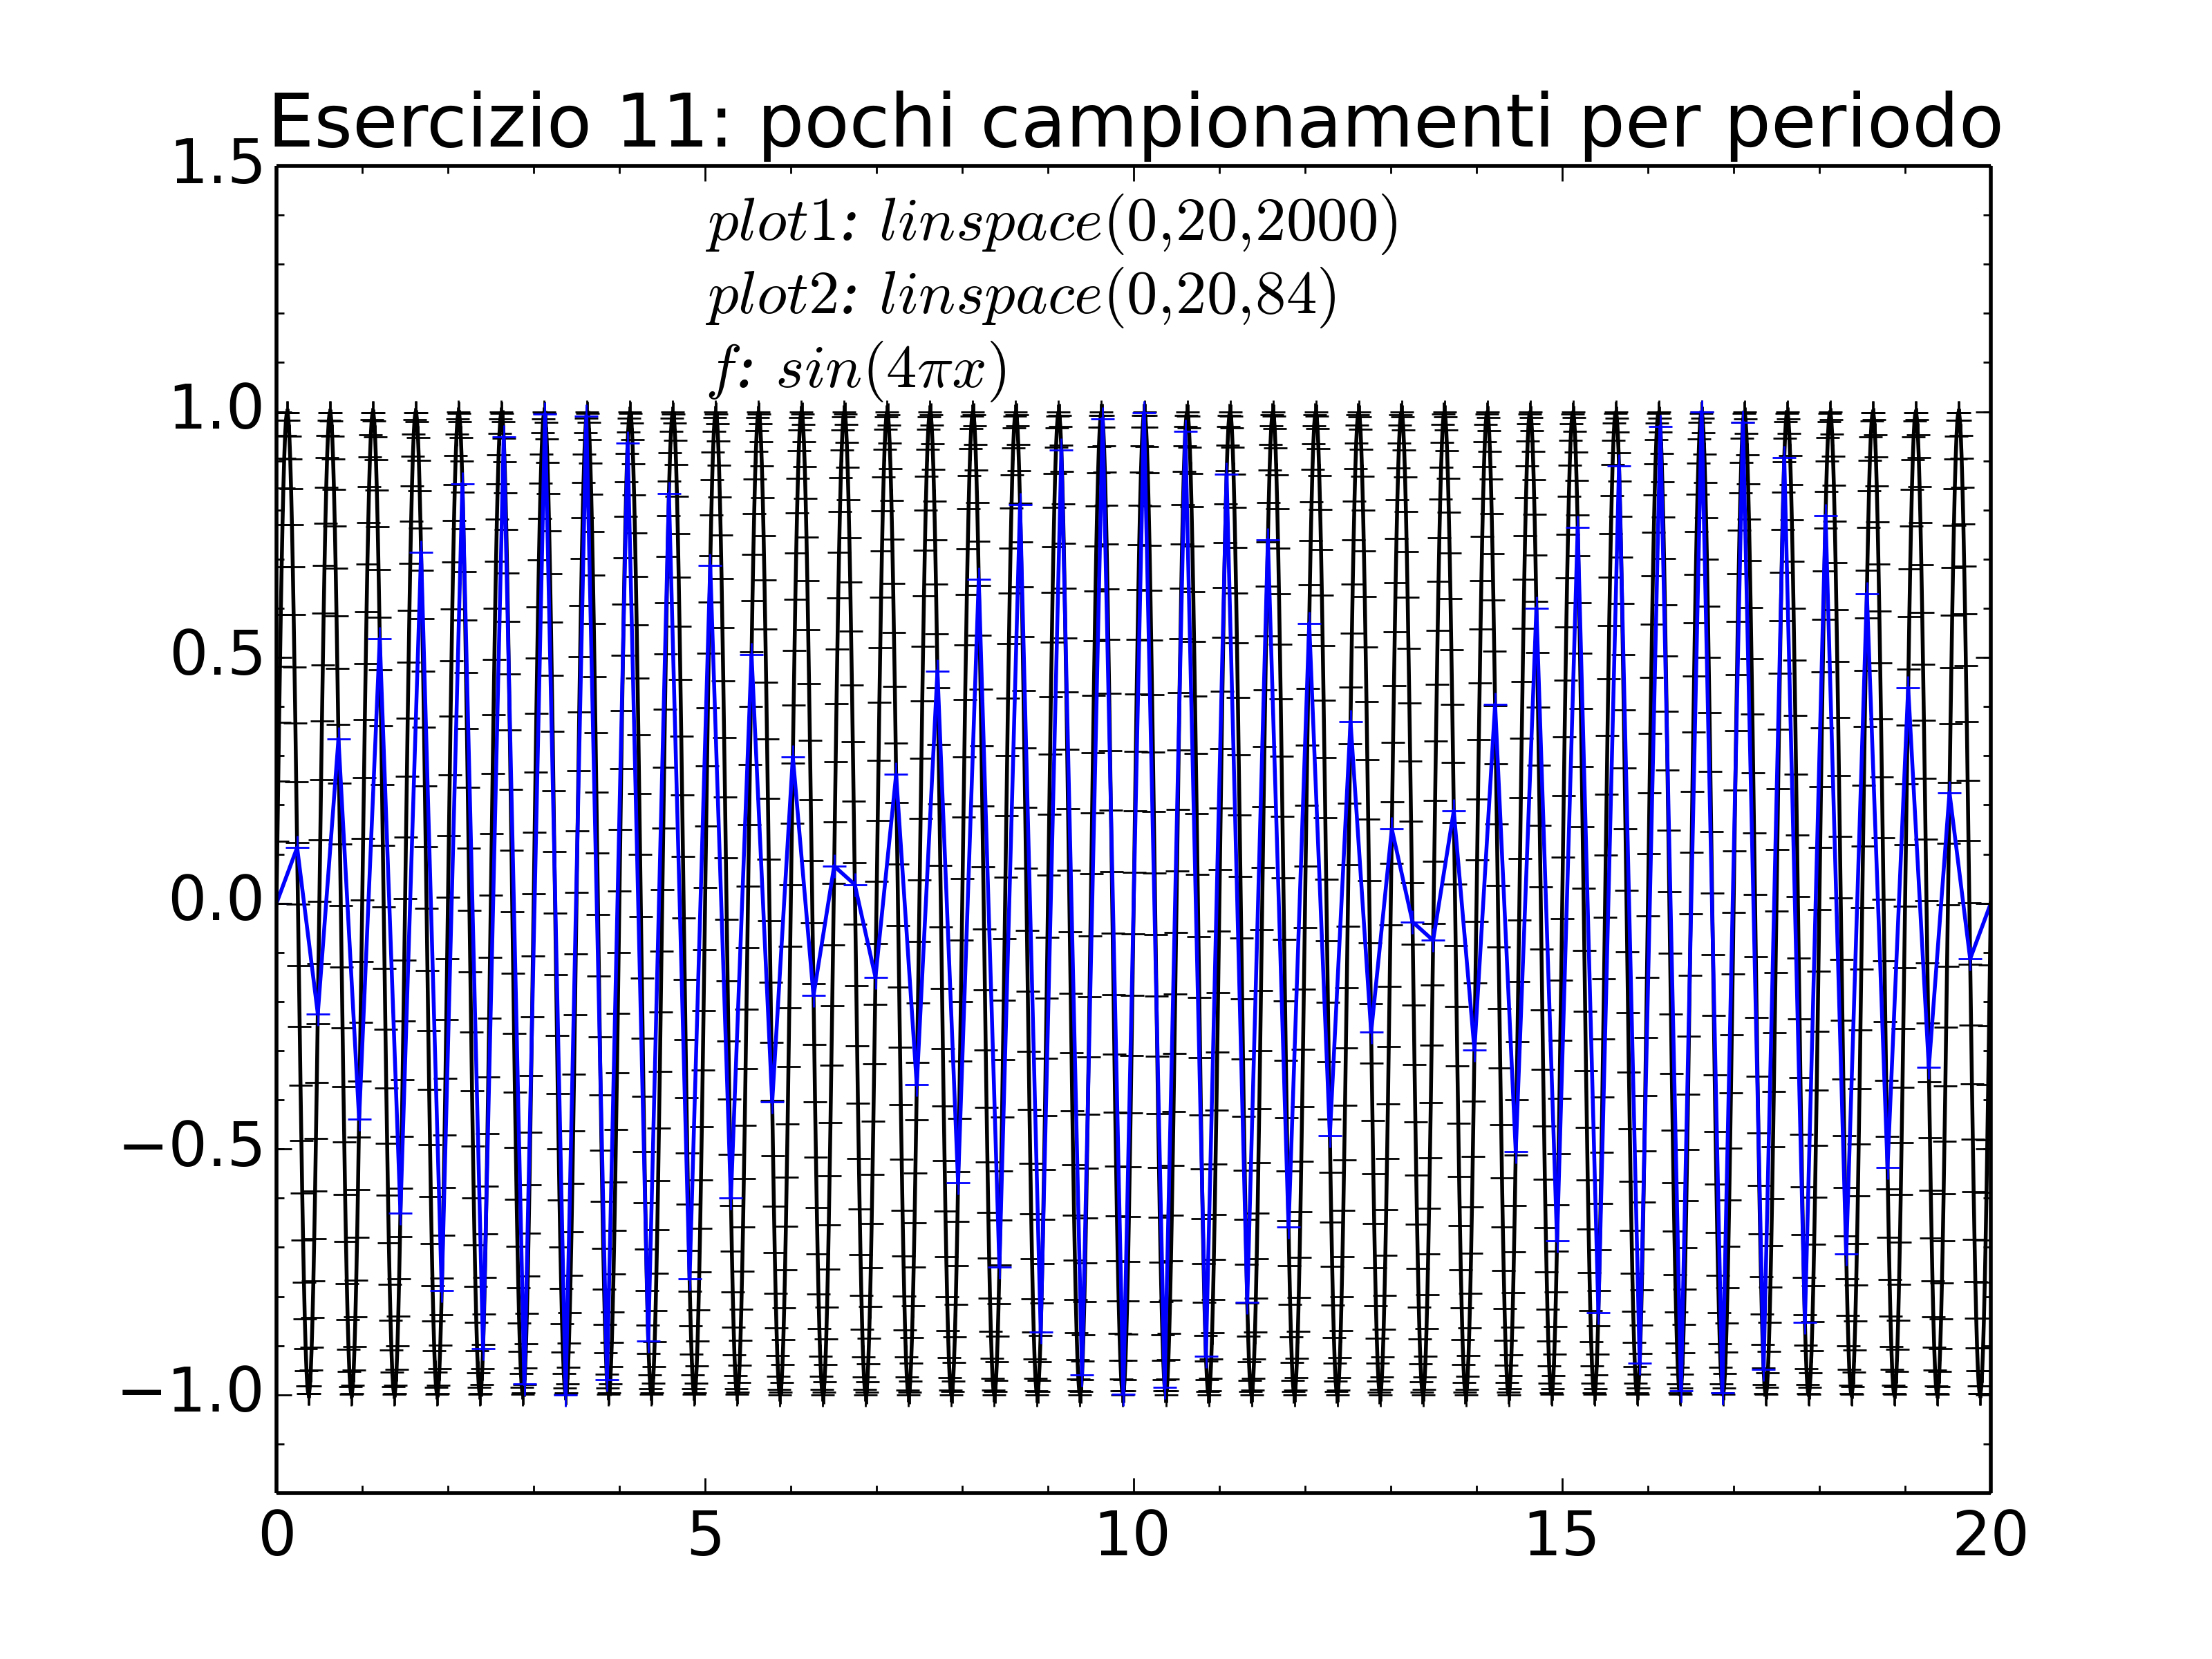
\includegraphics[width=0.9\linewidth]{./soluzione_es11_3batt}
\caption{Forma d'onda ottenuta dal campionamento di un segnale sinusoidale, acquisendo pochi dati per periodo}
\label{fig:soluzione_es11_3batt}
\end{figure}

Eliminiamo adesso l'istruzione di delay all'interno del void loop() dello sketch in uso e esaminiamo il risultato: per una frequenza di 1Hz il confronto fra l'acquisizione con il delay e senza il delay è immediato; la sinusoide, infatti, è ricostruita estremamente bene con circa 240 acquisizioni per periodo, invece che una decina. Un discorso analogo si può effettuare per frequenze di circa 4Hz: eliminando il ritardo scompare quell'artefatto simile ad un battimento. Per queste prime acquisizioni il \textit{baud} della porta seriale è stato lasciato costante a 9600bit/s. Questo, tuttavia, è solo uno dei due tempi in gioco nell'acquisizione delle tensioni tramite ARDUINO. Il primo è il tempo determinato dalla conversione del dato analogico in digitale e da tutte le operazioni e le istruzioni della routine di conversione, solo in un secondo momento il dato digitale viene inviato tramite la porta seriale, il cui baud potrebbe costituire un eventuale collo di bottiglia al procedimento complessivo di acquisizione e trasmissione del segnale. Notiamo intanto che, trascurando il tempo di conversione A $\rightarrow$ D, ad un baud di 9600 corrispondono circa 240 campionamenti al secondo, sia per $f=1$Hz che per $f=4$Hz, il che implicherebbe un numero di 40bit necessari per trasmettere una singola tensione (stringa di caratteri).\\

Vogliamo però capire se effettivamente i tempi di conversione sono trascurabili rispetto a quelli di trasmissione, o se invece compongono una parte rilevante del tempo totale. In prima analisi, ci aspettiamo che per baud sempre più alti ad un certo punto il numero di campioni per secondo tenda ad un valore costante, poichè, per quanto piccoli, i tempi di conversione sono comunque finiti e a quel punto costituirebbero un \textit{cap} al numero di campionamenti possibili per secondo. Se per baud relativamente bassi notiamo invece un aumento lineare del numero di campionamenti, allora si può concludere che è proprio il baud a costituire un cap (in questo range di funzionamento) al sampling rate. \\ Per verificare queste ipotesi, abbiamo effettuato diverse serie acquisizioni a frequenza costante di 4Hz, una per ogni baud disponibile nel VI \textsc{serial\_monitor}. Per calcolare il numero di campionamenti a secondo, sono state contate quante acquisizioni vi sono fra due massimi consecutivi (in un periodo), e moltiplicate per la frequenza. Nella tabella che segue sono riportati i dati in esame:\\


\begin{table}
\centering
\begin{tabular}{l|l|l}
\hline
\textbf{baud rate} & \textbf{ n.campioni/periodo}(4Hz) & \textbf{n.campioni/s} \\
\hline
9600 & 60(1) & 240(4)\\
14400 & 90(1) & 360(4)\\
19200 & 122(2) & 488(8)\\
38400 & 245(2) & 980(8)\\
57600 & 373(2) & 1492(8)\\
115200 & 748(3) & 2992(12)\\
\hline& 
\end{tabular}
\end{table}
~\\

Da questi dati è stato effettuato un fit lineare a due parametri, riportato in Figura (\ref{fig:es13_samples_vs_baud}).

\begin{figure}
\centering
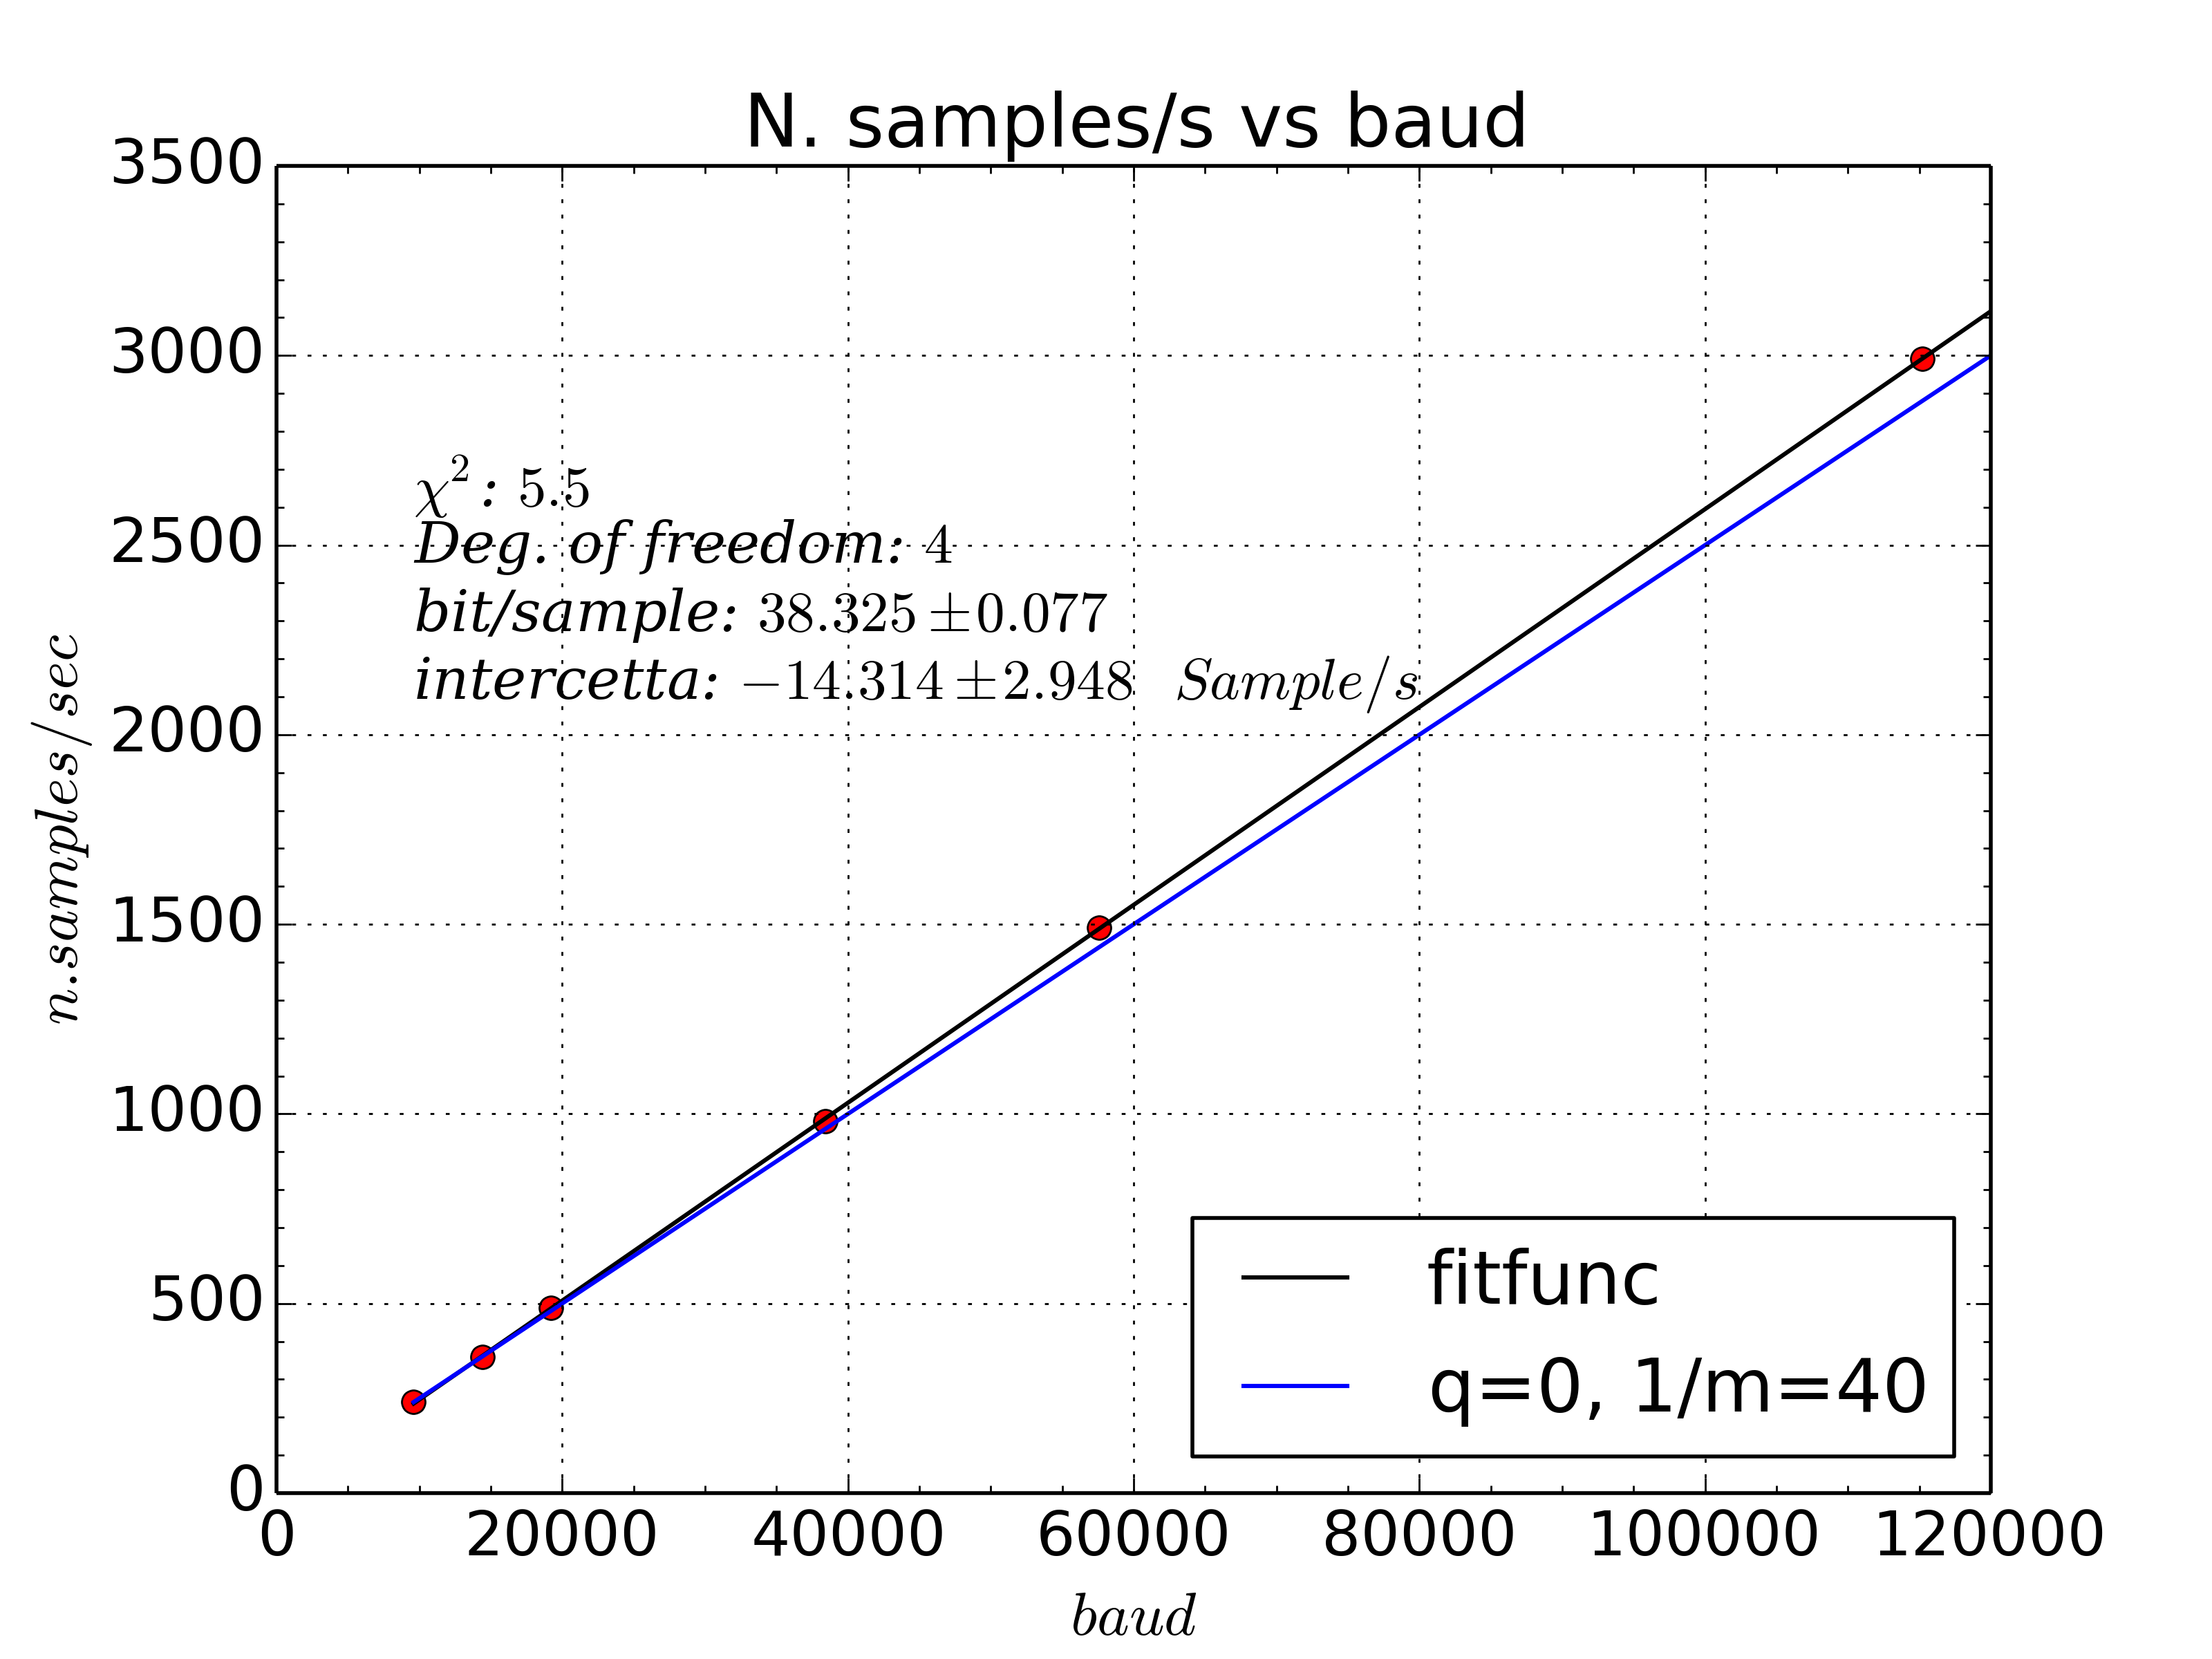
\includegraphics[width=0.9\linewidth]{./es13_samples_vs_baud}
\caption{Fit dei sampling rate vs baud: in nero la retta di fit con intrcetta libera, in blu la retta di tendenza corrispondente a intercetta nulla e pendenza di 40bit/dato}
\label{fig:es13_samples_vs_baud}
\end{figure}


Come è facile notare dal grafico, sembra che il sampling rate aumenti linearmente all'aumentare del baud, cosa che ci farebbe rientrare nella seconda ipotesi di partenza: quella cioè in cui è proprio il baud a fare da cap al sampling rate, e non i tempi di conversione e acquisizione delle tensioni. Infatti, ancora fino ad un baud = 115200 bit/s, non si notano scostamenti dal regime lineare. Questo dato ci permette di stimare un limte superiore al tempo di conversione:se fino al baud massimo il sampling rate aumenta linearmente, allora i tempi di conversione sono \textit{coperti} per tutte le scelte di baud, e in particolare saranno minori di $1/2992 s$, che è il reciproco del sampling associato al baud massimo, e che corrisponde quindi al tempo che intercorre fra un'acquisizione e l'altra. Da ciò si ottiene che i tempi di conversione devono necessariamente essere inferiori a $t_{sup} \simeq 330 \mu s$, che ci dà un utile limite superiore.\\

\subsection{Hw.2}
Per analizzare la regolarità del segnale acquisito con ARDUINO, si è proceduto ad un'analisi di Fourier discreta dei campioni per i vari baud scelti. I risultati sono visibili nel grafico di Figura (\ref{fig:multi_fft2}) e riassunti nella tabella riportata di seguito. Come misura dell'errore sulla frequenza, si è scelto il valore HWHM sul picco della componente più vicina ai 4Hz nominali. L'accordo dei valori delle frequenze è abbastanza buono: sono quasi tutte un po' inferiori al valore nominale (0.06-0.07 Hz in meno). Per quanto riguarda la dispersione, questa risulta maggiormente variabile fra i diversi baud, ma questa dipende essenzialmente dal numero di acquisizioni per ogni baud, che nel nostro caso non è stato mantenuto costante.

\begin{table}
\centering
\begin{tabular}{c|c|c}
\hline \textbf{baud} & $ f_{media}$ Hz & \textbf{HWHM} \\ 
\hline 115200 & 3.96 & 0.25 \\ 
57600 & 4.02 & 0.11 \\ 
38400 & 3.93 & 0.25 \\ 
19200 & 3.95 & 0.22 \\ 
14400 & 3.87 & 0.23 \\ 
9600 & 3.93 & 0.09 \\ 
\hline 
\end{tabular} 
\end{table}


\begin{figure}
\centering
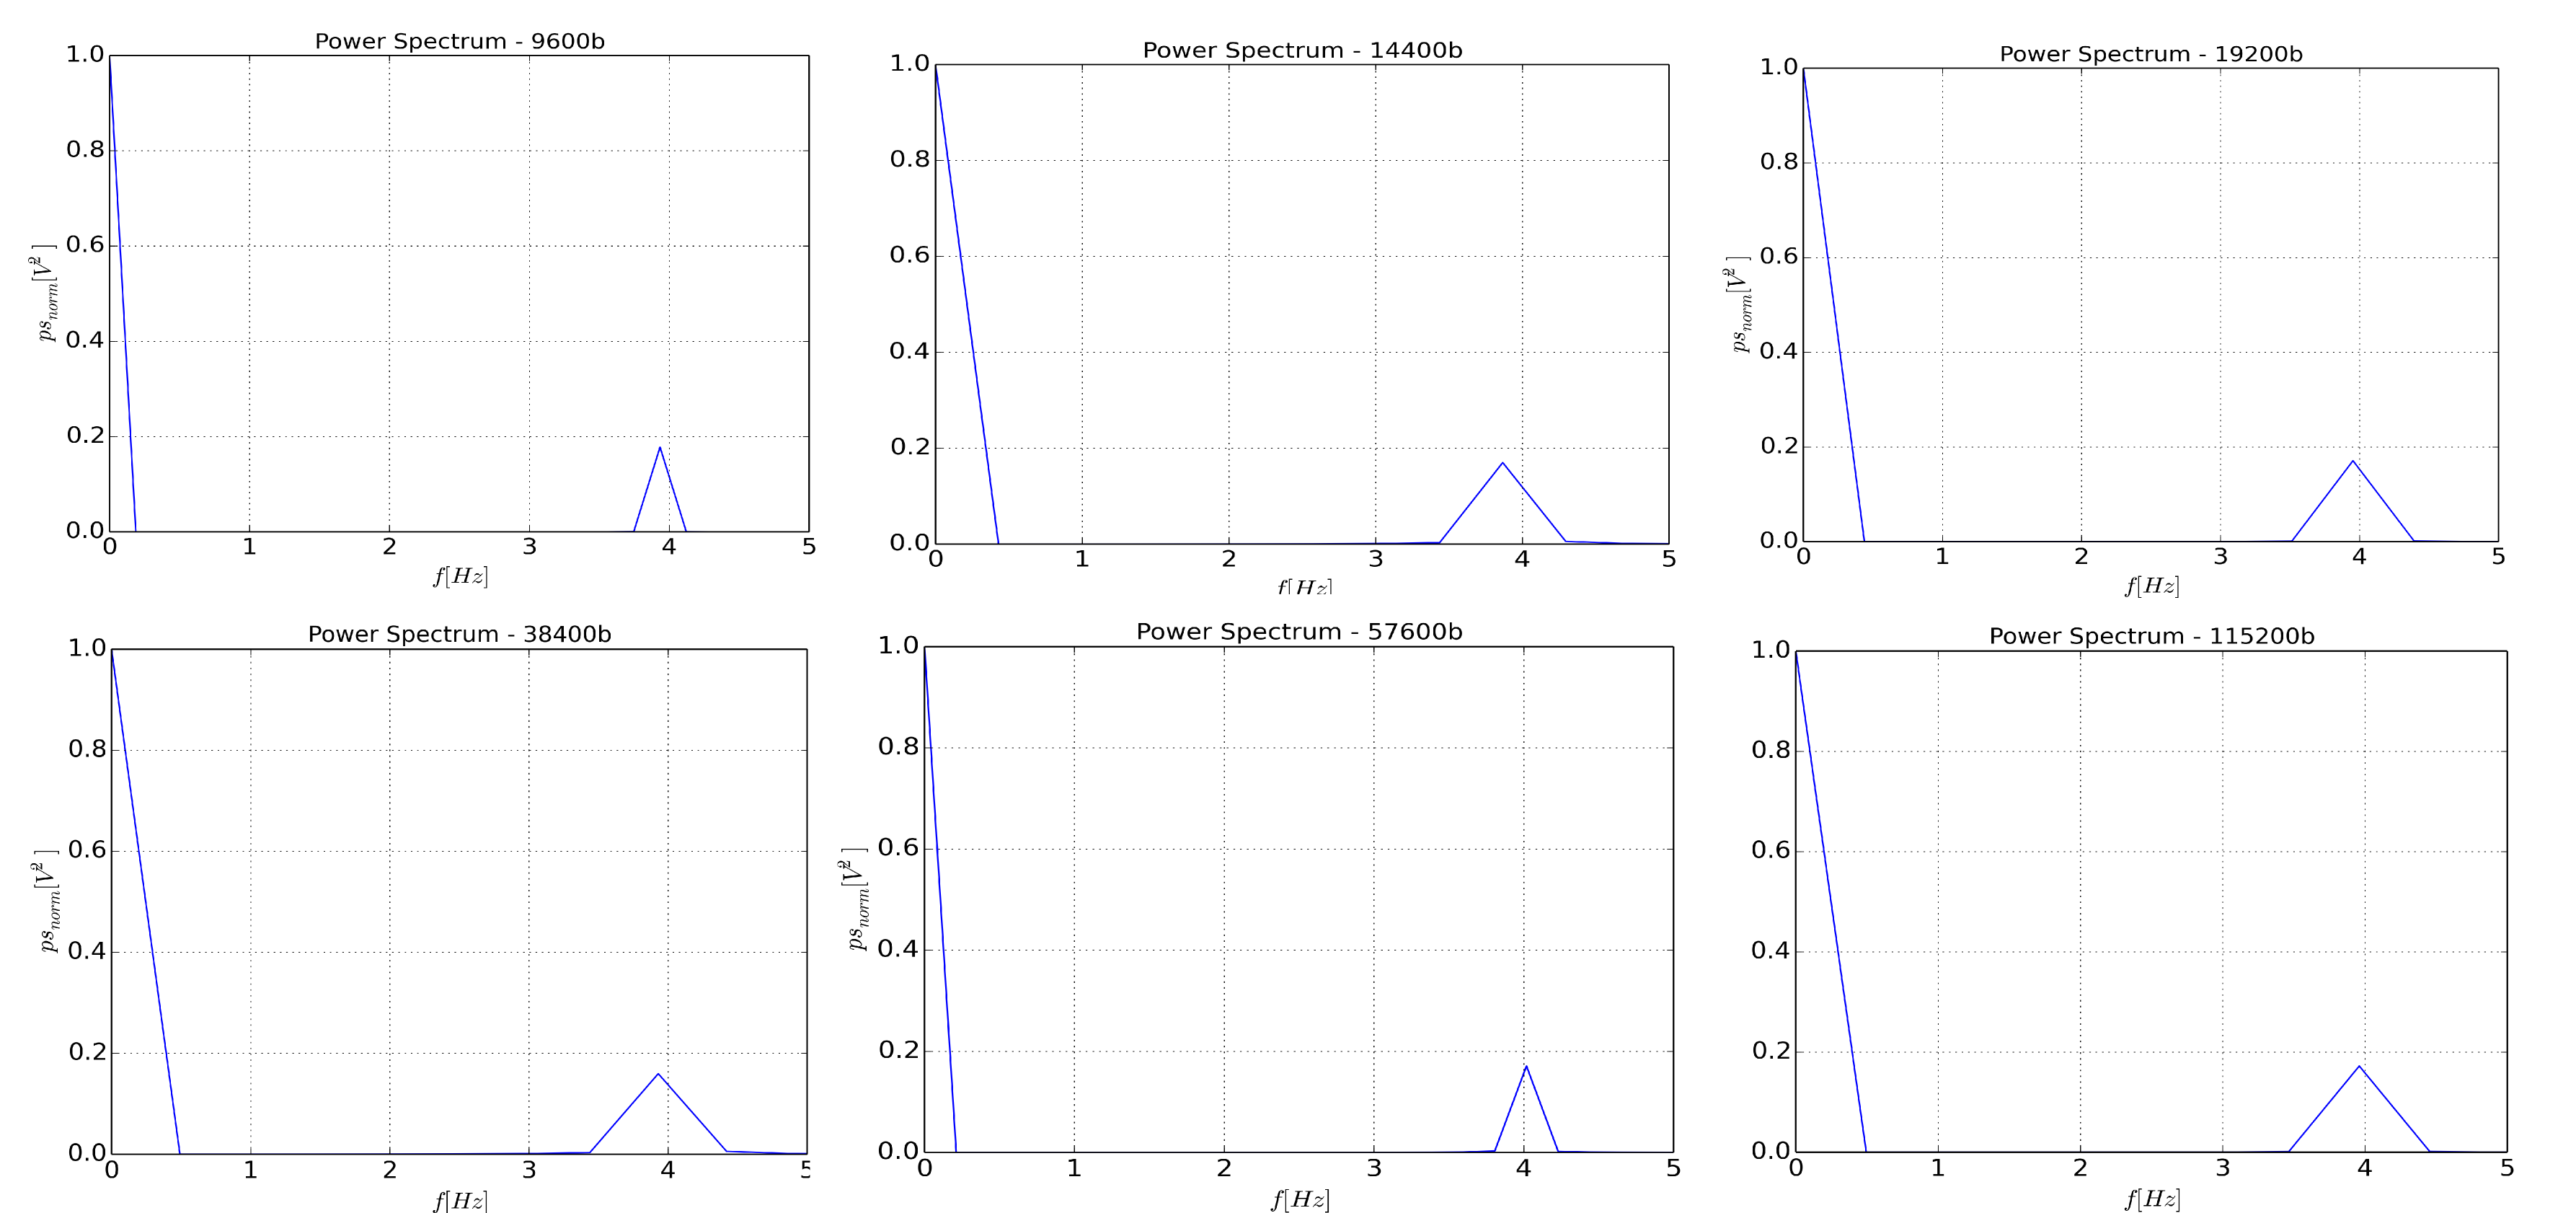
\includegraphics[width=1.1\linewidth]{./multi_fft2}
\caption{Multi plot: analisi di Fourier}
\label{fig:multi_fft2}
\end{figure}


\subsection{Onda triangolare}
Vorremmo analizzare più in dettaglio la regolarità delle acquisizioni di arduino, e per far ciò impieghiamo un'onda triangolare di frequenza sempre di 4Hz, $V_{pp} = 4V$ e offset +2.5V. Il segnale acquisito da Arduino è riportato in Figura (\ref{fig:es14_triang}). Consideriamo ora una porzione del grafico relativa ad un fronte di risalita: come retta di riferimento è tracciata la congiungente fra il primo e l'ultimo punto in esame. Fra la retta di riferimento e i punti acquisiti è stata effettuato lo scarto quadratico (riportato sulla scala di destra), vedi Figura (\ref{fig:hw3_triang}).\\

\begin{figure}
\centering
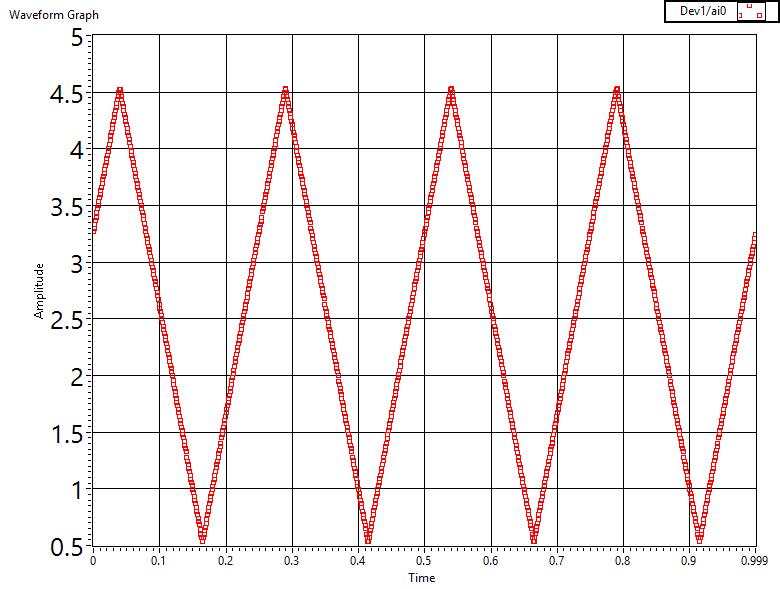
\includegraphics[width=0.9\linewidth]{./es14_triang}
\caption{Onda triangolare acquisita da Arduino}
\label{fig:es14_triang}
\end{figure}
 
 
 \begin{figure}
\centering
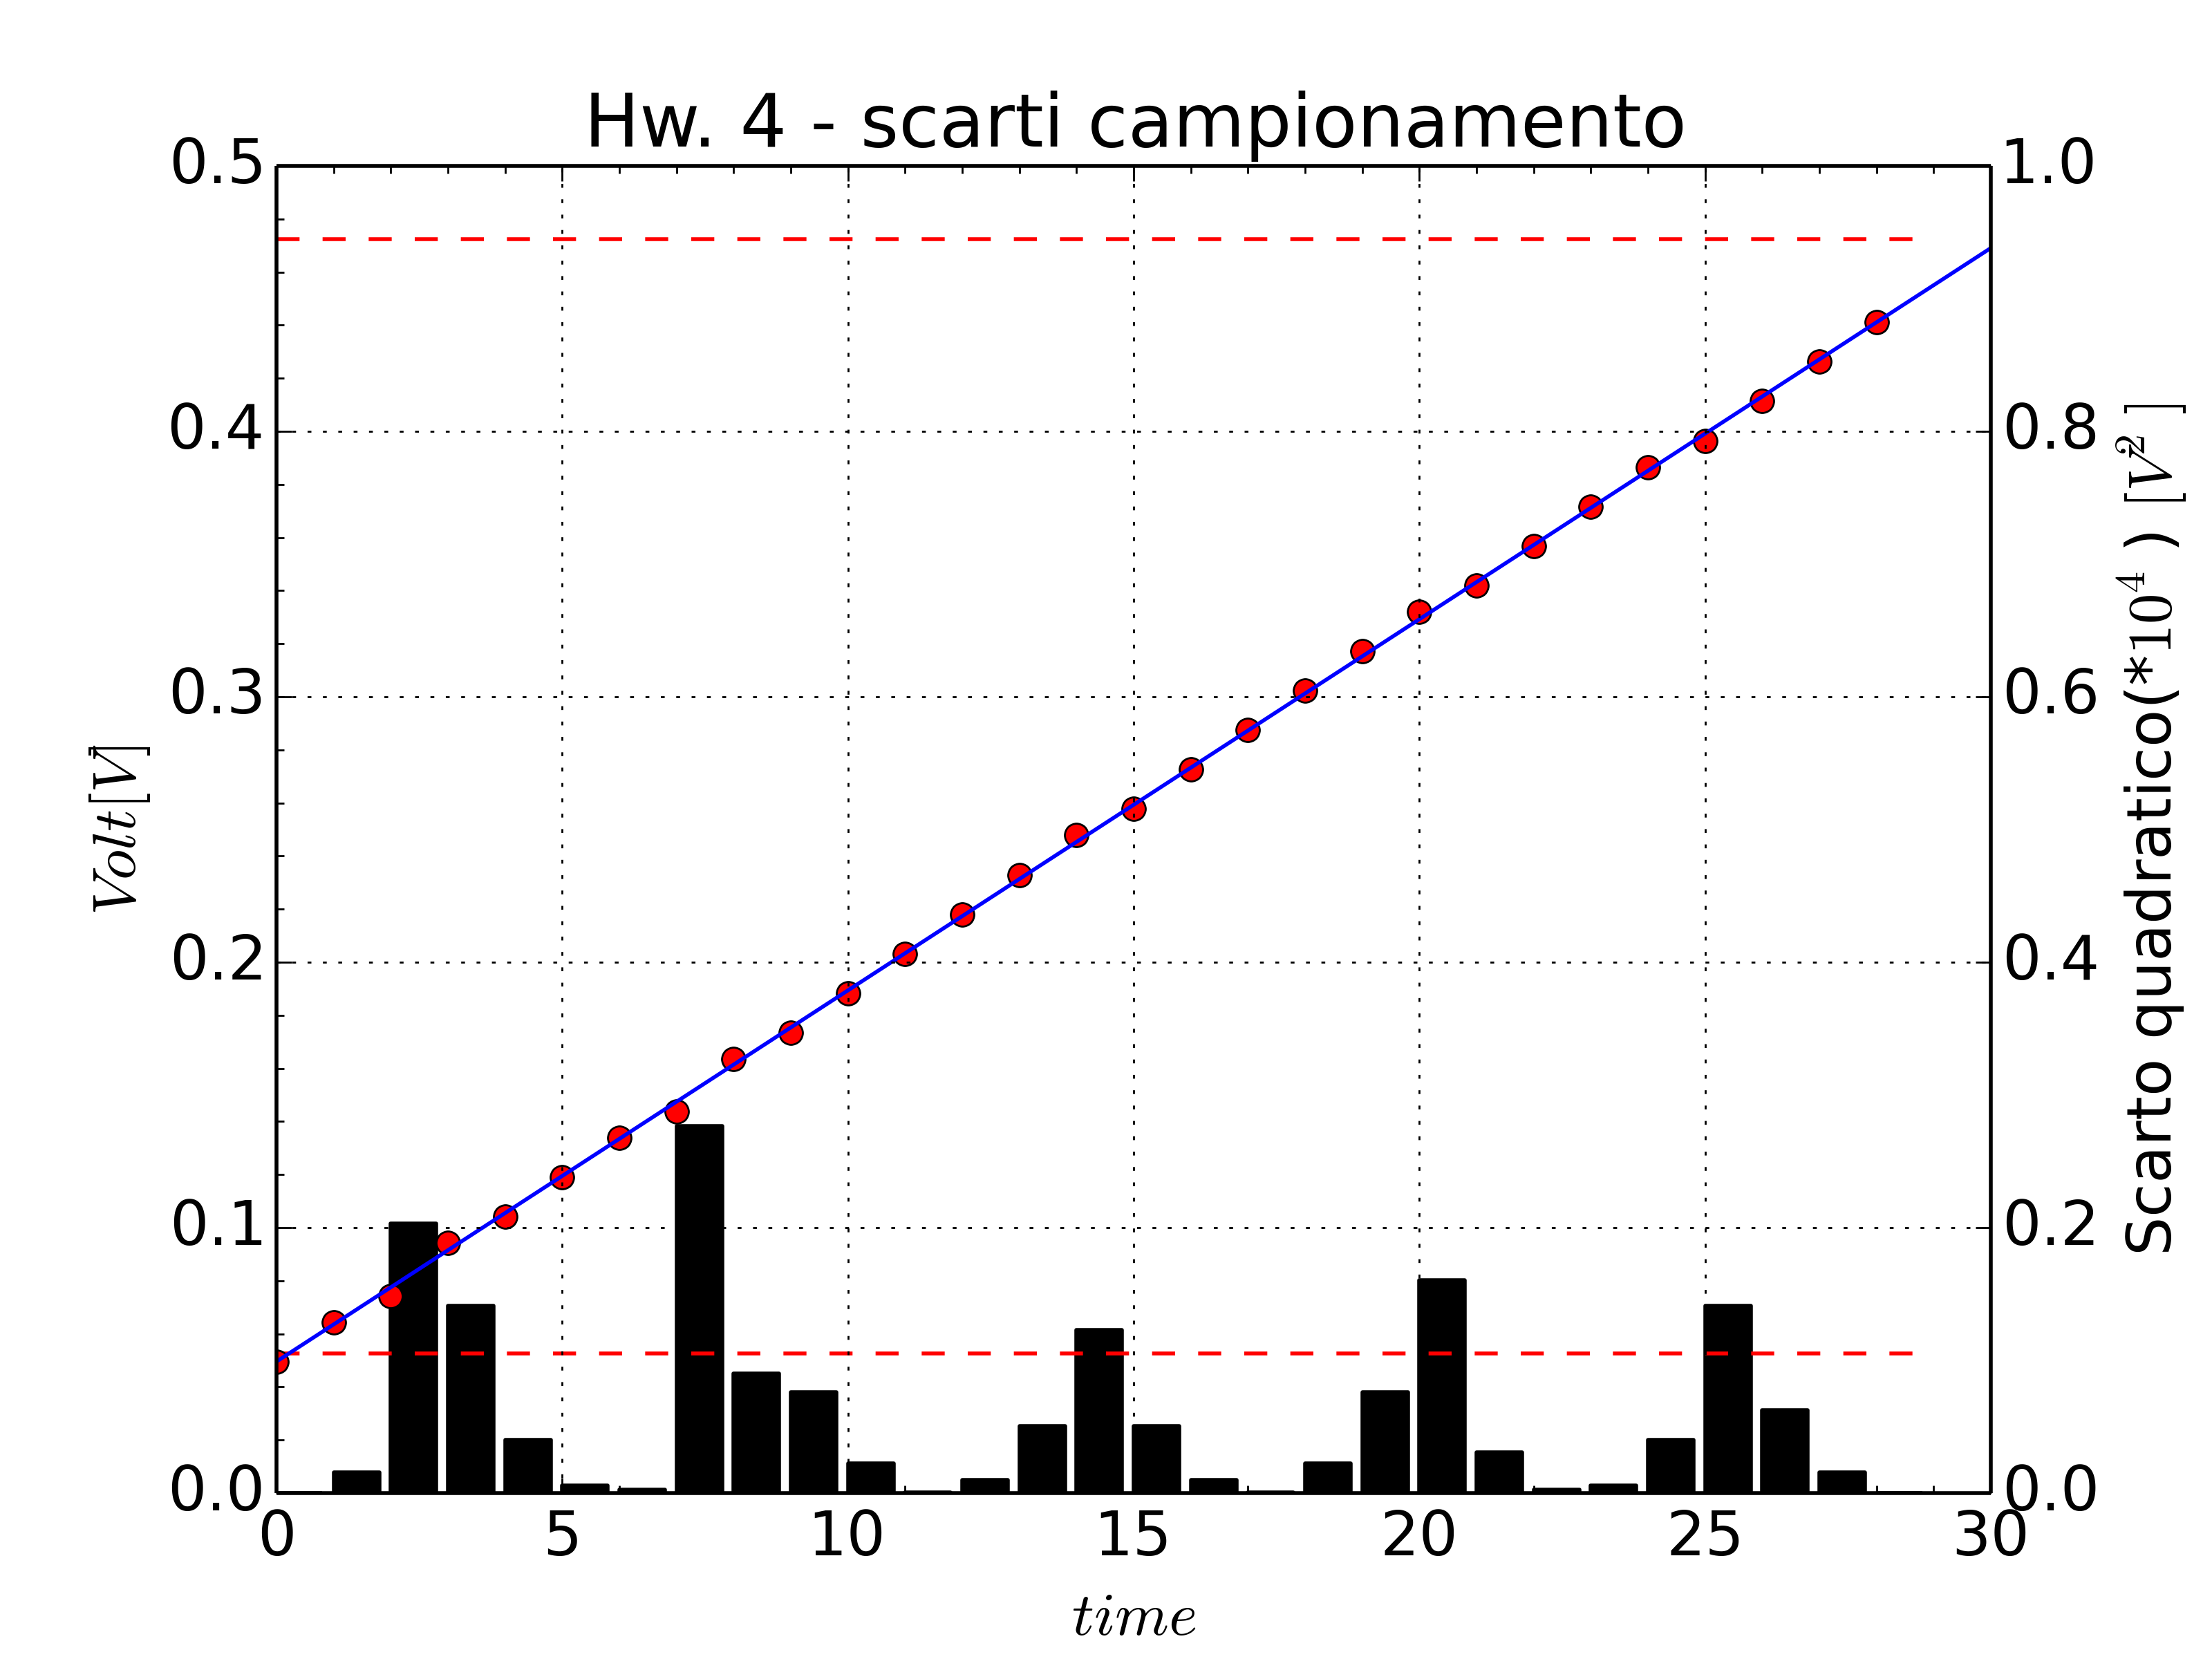
\includegraphics[width=0.9\linewidth]{./hw3_triang}
\caption{Regolaità della frequenza di campionamento}
\label{fig:hw3_triang}
\end{figure}

Si nota un certo pattern dei valori degli scarti, piuttosto regolare anche se dopo qualche ripetizione tende a sfasarsi. Un'ipotesi per spiegare questo risultato potrebbe coinvolgere la non regolarità delle acquisizioni rispetto ai livelli discreti che usa Arduino per misurare le tensioni, vale a dire: nell'intervallo di tempo necessario affinchè la tensione salga dal livello n $\rightarrow$ (n+1), Arduino esegue un numero frazionario di acquisizioni e si crea dunque uno sfasamento fra i due valori che si accumula, raggiunge un massimo e quindi decresce, per poi ricominciare nuovamente il ciclo dopo che si è ritornati alla situazione iniziale.

\section{Hw. 1 - AGGIORNAMENTO}
Come è visibile nello schema del convertitore ADC dell'ATmega328, la frequenza di campionamento di un segnale analogico non è direttamente quella di clock (20MHz), bensì quella che risulta dall'azione di un \textit{prescaler} sulla frequenza di partenza. Per il microcontrollore in nostro possesso, risulta un prescaler a 7bit, che divide la frequenza di clock, come impostazione predefinita, di un fattore 128. Di conseguenza, il clock input dell'ADC è circa 156kHz (20MHz/128). \\

Sapendo questo dato, è importante ora considerare la modalità con cui vengono eseguite le conversioni da analogico a digitale. Il modo più semplice, ma anche quello più oneroso dal punto di vista computazionale, è il cosiddetto '\textit{ramp} ADC': vi è quindi una sorta di rampa costituita dai successivi valori da 0 a 1023 (il nostro ADC è a 10bit di precisione), e ad ogni ciclo di clock viene eseguito un confronto fra la tensione sul pin ADC e il valore di riferimento, rendendo necessari un numero massimo di 1023 cicli per leggere ogni tensione. \\
Il secondo metodo è il '\textit{flash} ADC' che prevede l'avere a disposizione esattamente 1023 comparatori, settati a delle tensioni di riferimento crescenti, che leggono contemporaneamente l'ingresso, determinando dopo un solo ciclo di clock il valore convertito. Lo svantaggio di questo approccio è ovviamente l'elevato numero di componenti che, specialmente ad alte precisioni, rende l'ADC costoso e ingombrante. \\
Il terzo approccio, che è quello che usa il nostro chip, è il metodo per 'successive approssimazioni' (SA-ADC) che produce il risultato della conversione, idealmente dopo un numero di cicli di clock pari alla precisione (per noi, 10 cicli). Il funzionamento è semplice: nel primo step si controlla che l'input sia maggiore o minore del bit più significativo (MSB), $2^9 = 512$ (il conto dei bit va da 0 a 9), in caso affermativo viene scritto 1, altrimenti 0, e a questo valore diamo il nome $a_9$. Nel secondo step, si controlla se l'input sia maggiore di $a_9 2^9 + 2^8$, che dà come risultato 768 o 256, a seconda del confronto nel primo step, e il risultato lo chiameremo $a_8$. Nel terzo step si confronta l'input con $a_9 2^9 + a_8 2^8 + 2^7$ e si continua così fino ad ottenere al decimo passo la sequenza $a_9 a_8 a_7 ... a_0$ che coincide proprio con l'input. \\

Il numero di cicli di clock necessari per convertire un valore di tensione è dunque 10. Tuttavia, l'ADC si riserva qualche operazione in più, e complessivamente il numero di cicli dovrebbe essere 13. Questo significa che il sample rate sarà circa di 20MHz/128/13 = 12kHz. Secondo il Teorema del campionamento di Nyquist-Shannon, se un segnale ha spettro in frequenza limitato da una frequenza massima $f_{max}$, la frequenza di campionamento minima necessaria a ricostruire univocamente il segnale di partenza senza distorsioni è $2f_{max}$, il doppio di quella massima. Ciò significa che potremmo ottenere un buon campionamento di segnali a frequenza 5-6kHz, come ad esempio i segnali telefonici su rame che avevano una banda di circa 300-3300 Hz. Tale sampling è buono per campionare praticamente ogni strumento musicale: ad esempio un pianoforte tipico ha un'estensione di frequenza massima fino a 4200Hz circa.\\
Ovviamente, un modo per innalzare di molto la frequenza di sampling rate è quello di diminuire il fattore di prescaling: portandolo a 16 (ma anche a 32), otterremmo un sampling di 96kHz, più che adeguato per campionare qualunque suono appartenente alla frequenza uditiva umana ($f_{max} \simeq 20$kHz, ottimisticamente.)


\begin{thebibliography}{5}

	%Each item starts with a \bibitem{reference} command and the details thereafter.
	
	\bibitem{JH6} % Conference paper
	Product data sheet: Dual Type D Flip-Flop \textsc{mc14013b}.
	\url{http://onsemi.com}

	\bibitem{M06} % Conference paper
	Paul Horowitz, Winfield Hill - The Art of Electronics. Cambridge University Press (1989).
	
\end{thebibliography}


\end{document}